\documentclass[a4paper,11pt, uplatex]{ujreport} % A4,11pt標準 for uplatex
\usepackage[top=30truemm,bottom=30truemm,left=30truemm,right=30truemm]{geometry}

\usepackage[dvipdfmx]{graphicx}
\usepackage[dvipdfmx, colorlinks=true, linkcolor=blue, citecolor=red, filecolor=black, urlcolor=blue]{hyperref}
\usepackage{amsmath,amssymb}
\usepackage{cleveref}
\usepackage{threeparttable}
\usepackage{enumerate}


%% subcaptionを使うためのもの
\makeatletter
\let\MYcaption\@makecaption
\makeatother

\usepackage{subcaption}
%\captionsetup{compatibility=false}      % 必要に応じて

\makeatletter
\let\@makecaption\MYcaption
\makeatother


\usepackage[left]{lineno}
%\pagewiselinenumbers
%% 行間を2倍
%\renewcommand{\baselinestretch}{2}
%\doublespacing

% コマンド類
\newcommand{\fknee}{$f_{{\rm knee}}$}
\newcommand{\he}{$^3{\rm He}$}
\newcommand{\Pint}{$P_{{\rm int}}$}
\newcommand{\Pread}{$P_{{\rm read}}$}
\newcommand{\ctext}[1]{\raise0.2ex\hbox{\textcircled{\scriptsize{#1}}}}

\renewcommand{\bibname}{参考文献}
\renewcommand{\baselinestretch}{1.1}


\begin{document}

% 表紙
\thispagestyle{empty}
\begin{center}
\vspace*{1cm}
{\LARGE {\bf {\rm 修士論文} } }\\
\vspace*{1.5cm}
\setlength{\baselineskip}{1cm}
%{\LARGE {\bf {\rm CMB観測実験に用いる超伝導検出器~MKID~のノイズ低減を行うための評価環境開発研究}}}\\
%{\LARGE {\bf {\rm CMB観測実験で用いる超伝導検出器MKIDの評価研究}}}\\
{\Large {\bf {\rm CMB観測実験GroundBIRDの焦点面検出器アライメントと\\
長期運用に向けた角度データ取得システムの最適化
% CMB観測におけるベースラインゆらぎの抑制研究
}}}\\
%{\LARGE {\bf {\rm CMB偏光観測実験GroundBIRDで用いる\\高透過率真空窓の開発研究}}}\\
\vspace{1.5cm}
{\Large 京都大学 理学研究科 物理学・宇宙物理学専攻}\\
%\vspace{0.01cm}
{\Large 物理学第二教室 高エネルギー物理学研究室}\\
\vspace{1.5cm}
{\Large 片岡~敬涼}\\
%\vspace{0.5cm}
\vspace{0.5cm}
{\Large 2025年1月 24日}
\begin{figure}[h]
 \centering
 
\includegraphics[width=0.6\columnwidth]{0_title/E-C.png}
\end{figure}


%\vspace{3cm}
%{\Large 2019年1月2日}

\end{center}
 
%

% abstract
\newpage
\begin{abstract}
\hspace{-4mm}

%gaiyou(CMBで迫りたい物理(ニュートリノ質量和、tau)、GB、自分のやったことがどう重要なのかを簡潔に記す)
宇宙マイクロ波背景放射(CMB)の温度異方性の観測によって、宇宙の進化を記述する標準理論が構築されてきた。現在ではCMBの偏光観測が大きなテーマとなっており、偏光を通してインフレーション理論やニュートリノ質量和、宇宙の再電離といった課題に迫ることができる。

GroundBIRDはスペイン領テネリフェ島の標高2,400 mに位置する大角度スケールの観測に特化した地上CMB望遠鏡である。望遠鏡を1分間で20回転させる高速スキャンによって大気揺らぎの影響を抑制した観測を行う。高速スキャンがもたらす効果を最大限に発揮するために、時間応答性の良い超伝導検出器MKIDを焦点面検出器として採用し、2023年5月から本格的な観測を開始した。大角度スケールでの偏光Eモードを観測することで、宇宙再電離期を特徴付け、さらにニュートリノ質量和と縮退したパラメータである光学的厚み$\tau$を誤差$\sigma_{\tau}\sim 0.01$で測定することを目指している。

観測を続けてデータを蓄積する段階にある現在、安定して長期運用をすること、そして質の良いデータを取得することが要求される。しかし、本研究の開始前の観測システムにおいて2つの未解決課題があった。1つは望遠鏡仰角データ取得システムが硬直的であること、もう1つは天球上での検出器配置がスキャン軸から傾いていることである。本論文ではこれらの課題に対する改善と最適化を行なった。

仰角データの取得にFPGAボードを使用しているが、人手を必要とするメンテナンスを高頻度で要し、システム運用をリモート主体で行えないことが、長期運用に対する障壁となっていた。本論文ではボード内のFPGAチップにPYNQと呼ばれるOSシステムを搭載し、OS上からソフトウェアを動かすことでデータ取得の操作性向上とアクセス性の向上を図ることにした。本研究でこのシステムを開発し、望遠鏡にインストールし、信号処理の確認と安定動作を確認した。

焦点面に搭載した多数のMKIDによってCMBの偏光信号を検出する。ここで、無偏光な大気放射ノイズを抑制するためにスキャン軸上の異なるMKID間で信号の差分をとる。しかし、スキャン軸とMKIDの配置軸に傾きがあると差分をとっても大気放射ノイズを十分に差し引けない。本研究では、月の観測データからこの問題を定量的に洗い出した。具体的には、MKIDの配置軸が望遠鏡のスキャン軸に対して約6°傾いていることを見積もった。そして、この結果をもとに、焦点面を含む望遠鏡の構造体を回転させることで天球上でのMKIDの配置軸を改善した。本研究ではさらに月と木星の観測データからこの改善の確認も行なった。加えて、スキャン軸上に配置されているMKID間で信号差分をとり、各入射信号の相関の強さを示す指標に焼き直し、回転の前後で比較することで観測する大気の揺らぎを抑制する結果を得た。

以上2点の改善と最適化を通してGroundBIRDが持つ運用、観測性能の向上を成功させた。



%本論文の構成を述べる。第\ref{chapter1}章でCMBに関わる理論的な背景、第\ref{chapter2}章でGroundBIRD実験の概要を説明する。以降は第\ref{chapter3}章と第\ref{chapter4}章の2部構成になっており、第\ref{chapter3}章でGroundBIRDの角度データ取得システムの改善について、第\ref{chapter4}章で焦点面検出器のアライメント較正とその結果について述べる。第\ref{chapter5}章で今後の展望を述べ、第\ref{chapter6}章でまとめを述べる。


\end{abstract}


%\thispagestyle{empty}
%

% 目次
\newpage
\pagenumbering{roman}
\setcounter{page}{1}
\setcounter{tocdepth}{2}
\tableofcontents
%\listoffigures
%


% 本文
\newpage
\pagestyle{headings}
\pagenumbering{arabic}
\setcounter{page}{1}
\setlength\floatsep{0pt} %dblfloatsep		%ページの上下に出力される図と図の間のスペース
\setlength\abovecaptionskip{0pt}	%図とキャプションの間のスペース


%
\chapter{序論}

宇宙マイクロ波背景放射({\bf C}osmic {\bf M}icrowave {\bf B}ackground radiation)~は人類が観測できる最古の光である。
これまでに、その温度異方性の精密観測によって現在の宇宙論の基礎が確立された。
現在では~CMB~の偏光観測に焦点が当てられており、宇宙の成り立ちを解き明かそうと様々な実験が進められている。
本章では~CMB~と宇宙論についての概要を述べた後に、CMB~偏光観測実験~GroundBIRD~について述べる。
最後に本研究の動機と本論文の構成について述べる。

\section{~CMB~の温度異方性と標準宇宙論}
CMB~の周波数スペクトルがほぼ~2.725~K~の黒体放射のスペクトルと一致することが測定され\cite{cobe,cmb_discovery,cmb_discovery_theory}、
宇宙初期は熱平衡状態であったことが証明された。
そして~CMB~の精密観測によって、宇宙の時間発展を記述する標準モデルである「$\Lambda$-CDM~モデル」が構築され、そのパラメータの決定精度が年々向上している\cite{plank}。
一方で、未解決の課題もある。例えば最終散乱面時刻までに
宇宙が相関を持てる領域は視野角にしてわずか~$2^\circ$~であるにもかかわらず、
あらゆる方向から到来する~CMB~の強度は十万分の一~($10^{-5}$)~の精度で同じである。
本節では~CMB~の温度異方性、現在の標準宇宙論とそれらの抱える問題点(地平線問題)について述べる。


\subsection{CMB~の温度異方性観測の歴史}
1996~年に~COBE~衛星によって~CMB~のスペクトルが~$2.725~{\rm K}$~の黒体放射のスペクトルと同じであることが測定された(図~\ref{cobe_plank}~左)。
このことは宇宙初期に物質と光とが熱平衡状態であったことを意味し、
高温・高密度の状態から宇宙が成長してきたというビッグバン宇宙論の観測的証拠となった。
また、COBE~は温度異方性も発見し、これは宇宙の大規模構造を作り出すタネである初期揺らぎの発見となった。
その後、CMB~の温度異方性の精密観測のために打ち上げられた~WMAP~や~Plank~衛星により、全天におけるCMBの温度異方性
の測定精度は$10^{-6}~{\rm K}$~まで向上した。

\begin{figure}[h]
  \begin{tabular}{cc}
    %---- 最初の図 ---------------------------
    \begin{minipage}[t]{0.5\hsize}
      \centering
      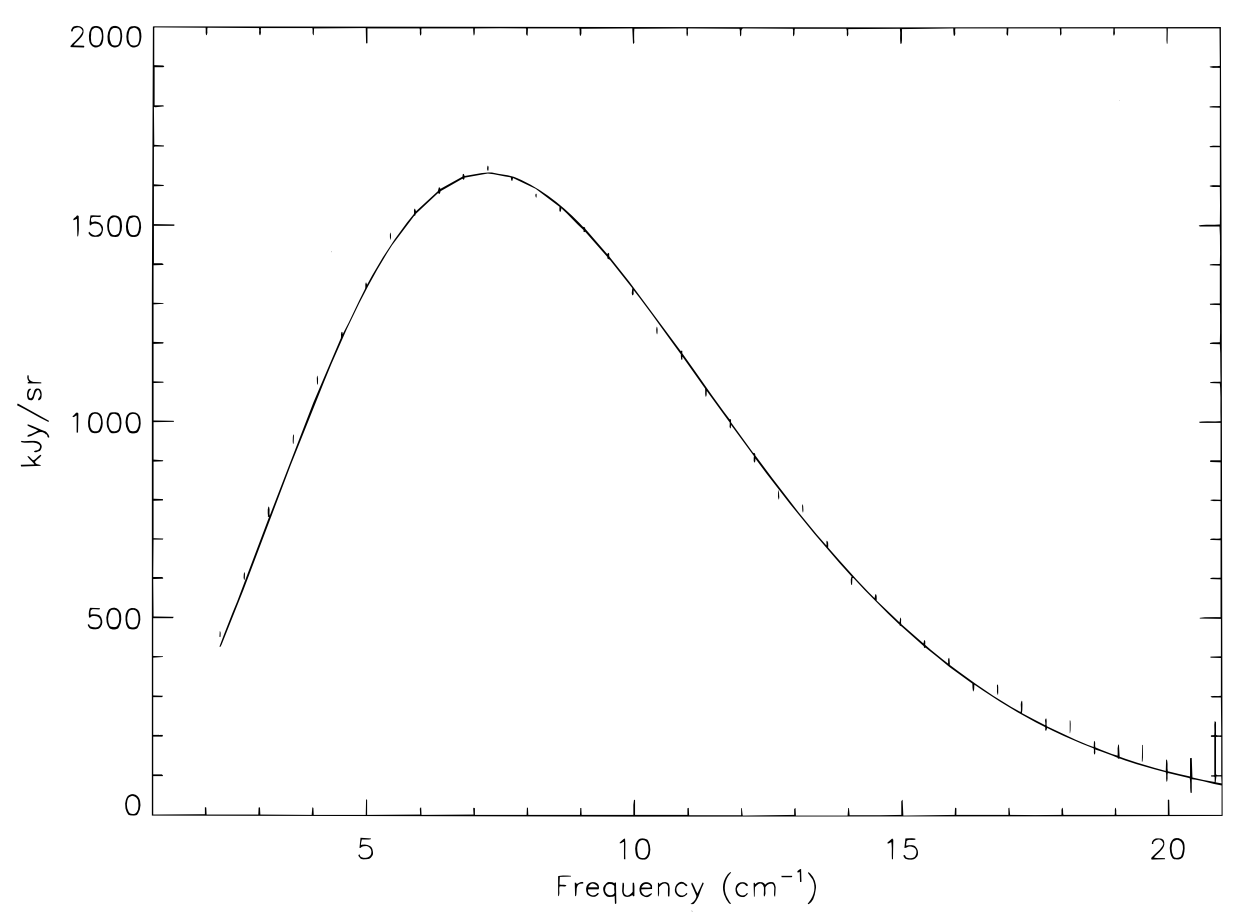
\includegraphics[keepaspectratio, scale=0.3]{2_cosmology/figs/cobe.png}
    \end{minipage} 
    %---- 2番目の図 --------------------------
    \begin{minipage}[t]{0.5\hsize}
      \centering
      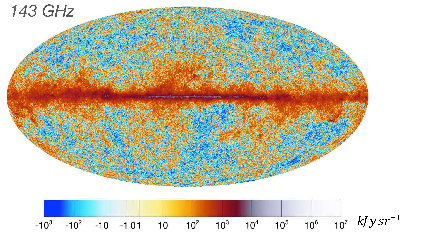
\includegraphics[keepaspectratio, scale=0.9]{2_cosmology/figs/plank_temp143.pdf}
    \end{minipage}
    %---- 図はここまで ----------------------
  %\caption{GroundBIRDの概要}
  \end{tabular}
  \caption{(左)COBE~衛星によって観測された~CMB~のスペクトル\cite{cobe}。
  この結果から~CMB~の温度が$2.717 \pm 0.007~{\rm K}$~ともとまった。
  (右)Plank~衛星によって観測された~143~GHz~における温度異方性のマップ\cite{plank}。}
  \label{cobe_plank}
\end{figure}

\subsection{CMBと宇宙論パラメータ}
宇宙が高温・高密度の時期は光は頻繁に散乱されるため、いわば不透明な状況であった。
宇宙膨張によって宇宙が冷えていくにつれて、光を散乱する電離イオンの数が減り、散乱確率が小さくなっていく。
宇宙の温度が~3000~K~ほどになると、トムソン散乱の断面積から計算される光の平均自由時間がその時刻におけるハッブル時間よりも長くなり、
光は電離イオンに散乱されずにまっすく進むようになる。この時期を宇宙の晴れ上がりと呼ぶ。
他にも、この時期を「最終散乱時刻」と呼ぶこともある。そして、最終散乱時刻に対応する動径座標を半径とする球核を「最終散乱面」と呼ぶ。

CMBの観測では図~\ref{cobe_plank}~の右図のような~CMB~強度分布を望遠鏡を用いて測定する。
その強度分布図を「マップ」と呼び、
マップを球面調和関数展開して得られるパワースペクトル($C_l$)から宇宙論を記述するパラメータを求めることができる。

図~\ref{kyumen}~のように、観測者を中心とする球座標で、観測者の視線方向を表す単位ベクトル~$\hat{n}$~を

\begin{equation}
  \hat{n} \equiv (\sin\theta \cos\phi , \sin\theta \sin\phi, \cos\theta)
\end{equation}

と定義する。

\begin{figure}[htbp]
  \centering
  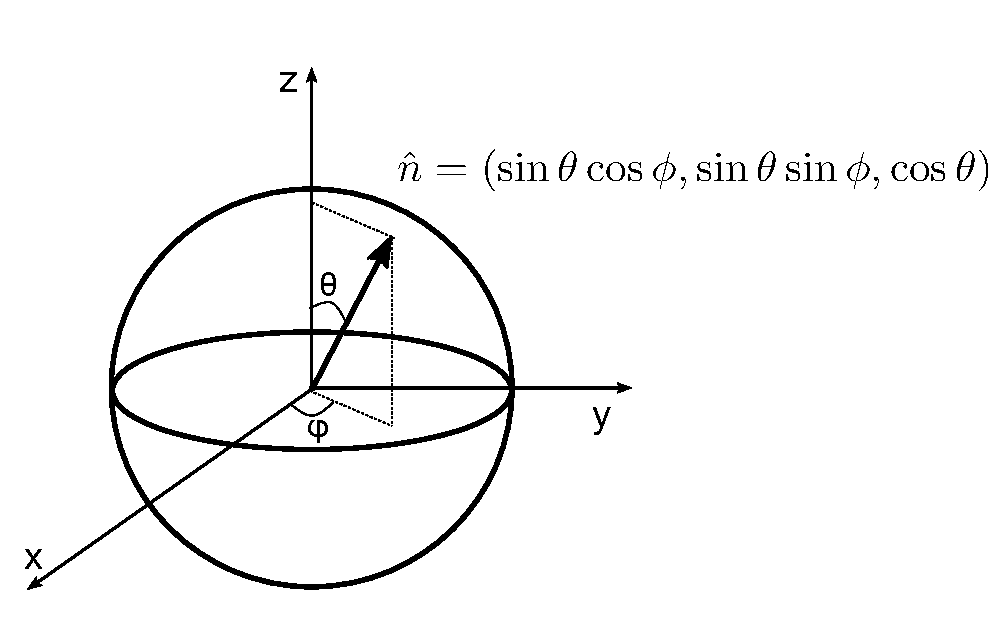
\includegraphics[width=0.6\columnwidth]{2_cosmology/figs/kyumen_all.pdf}
  \caption{デカルト座標と観測者を中心とする球座標}
  \label{kyumen}
\end{figure}

この座標系における~CMB~温度の平均値~($\bar{T}$)~からのずれ~$\Delta T(\hat{n}) \equiv T(\hat{n}) - \bar{T}$~を球面調和関数で
\begin{equation}
 \Delta T(\hat{n}) = \sum_{\ell=1}^{\infty}\sum_{m=-\ell}^{\ell}a_{\ell m}Y_\ell^m(\hat{n}).
\end{equation}
と展開する。$a_{\ell m}$~は展開係数である。添字の~$\ell$~は``Multipole"~と言い、全天における温度揺らぎのスケールの大きさを表す。
図~\ref{kyumen_plot}~のように、添字~$m$~に対応する軸に対して、全天を~$\ell$+1~の領域に分割すると領域の間隔~$\delta \theta$~は
\begin{equation}
  \delta \theta = 180^{\circ} /\ell
\end{equation}
で与えられる。つまり、ある~$\ell$~における異方性は、天球上で半波長の見込み角度が~$180^{\circ} /\ell$~程度となる分布を持つ。

\begin{figure}[htbp]
  \centering
  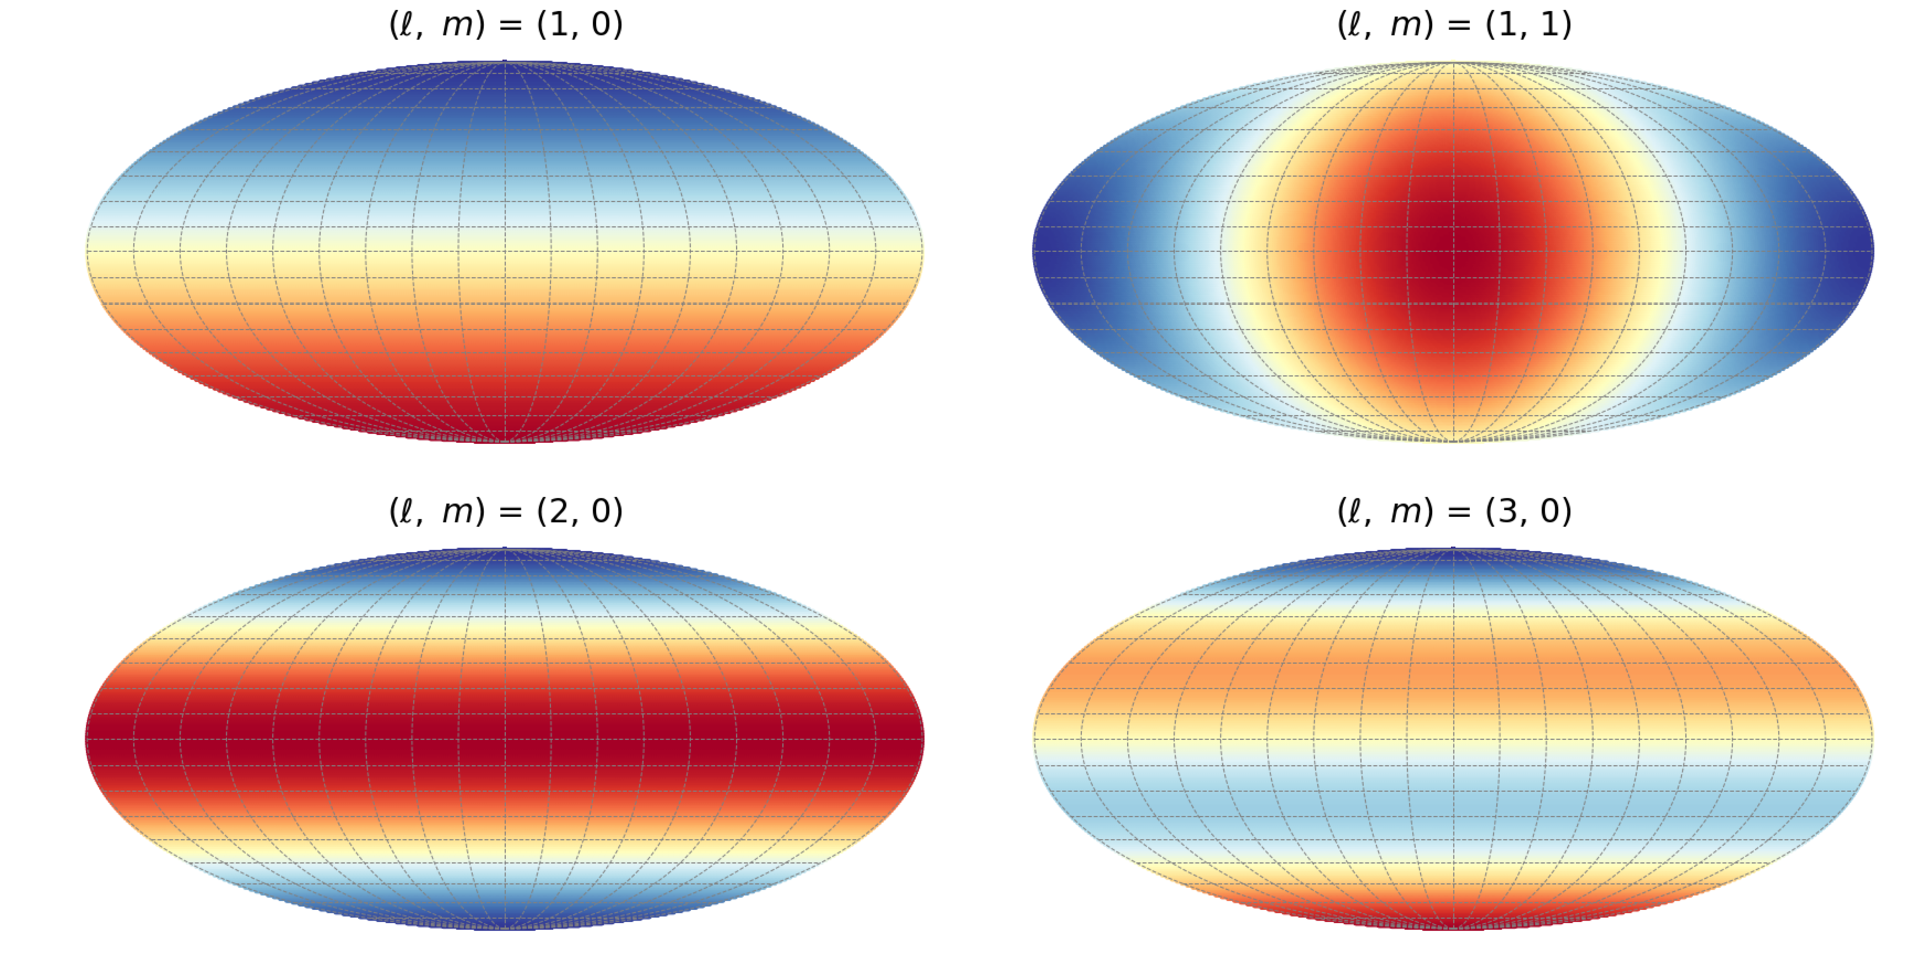
\includegraphics[width=1\columnwidth]{2_cosmology/figs/kyumen_plot.pdf}
  \caption{モルワイデ図法で表した球面調和関数の例。CMB~マップは、
  様々な~$\ell$~の球面調和関数を重ね合わせによって表現される。}
  \label{kyumen_plot}
\end{figure}



しかし、展開係数~$a_{\ell m}$~は添字~$m$~による方位角に依存しているため、座標の選び方によって値が異なる。
したがって、パワースペクトル~$C_\ell$~を展開係数~$a_{\ell m}$~を用いて
\begin{equation}
 C_l \equiv \frac{1}{2l+1}\sum_{m=-\ell}^{\ell}a_{\ell m} a_{\ell m}^* . \label{equ_cl}
\end{equation}
と定義する。この値を用いることで、座標原点によらない解析を行うことができる。
図~\ref{cobe_plank}~の右図のマップから計算されたパワースペクトルを図~\ref{plank_cltt}に示す。


また、このパワースペクトルから得られた宇宙論パラメータを表~\ref{plank_cospar}に~まとめる。
このように全天の温度異方性観測からパワースペクトルを計算し、後述する$\Lambda$-CDM~モデルのパラメータを数$\%$
の精度で求めることができている。
\begin{figure}[htbp]
  \centering
  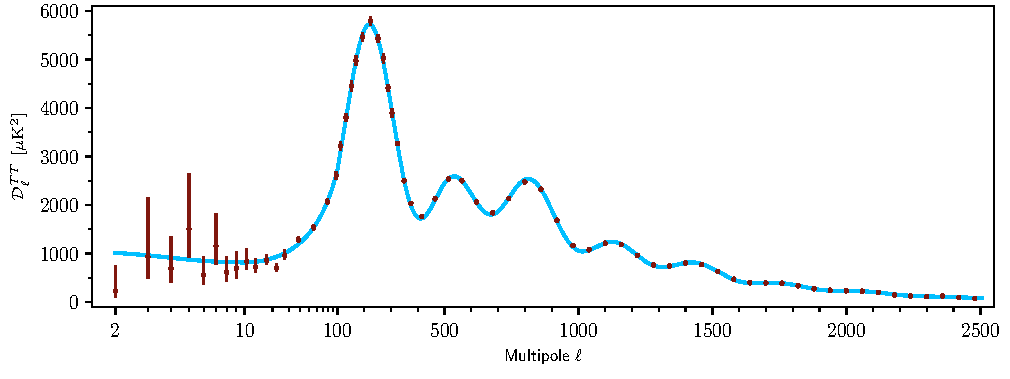
\includegraphics[width=0.9\columnwidth]{2_cosmology/figs/plank_cltt.pdf}
  \caption{Plank~の観測から計算された温度パワースペクトル\cite{plank}。
  $D_{\ell}^{TT}$~は~$D_{\ell}^{TT} = \frac{\ell (\ell +1) C_l}{2 \pi}$~である。}
  \label{plank_cltt}
\end{figure}

\vspace{2mm}
\begin{table}[htbp]
  \centering
  \caption{Plank~の観測から得られた$\Lambda {\rm CDM}$~モデルの宇宙論パラメータ\cite{plank}。
  これらの値の推定には偏光と~lensing~のパワースペクトルも用いる。}
  \vspace{2mm}
  \begin{tabular}{l|l}\hline
    $\Omega_b h^2$ ~(バリオン密度)& 0.02237 $\pm$ 0.00015 \\
    $\Omega_c h^2$ ~(CDM~密度)& 0.12011 $\pm$ 0.0012 \\
    $100 \theta_{MC}$ ~(最終散乱面の見込み角度) & 1.04092 $\pm$ 0.00031 \\
    $\tau$ ~(再電離期における光学的な厚さ)& 0.0544 $\pm$ 0.0073 \\
    $ln(10^{10}A_s)$ ~(スカラー型の原始揺らぎの振幅) & 3.044 $\pm$ 0.014 \\
    $n_s$ ~(スカラー型の原始揺らぎのべき係数)& 0.9649 $\pm$ 0.0042 \\ \hline
  \end{tabular}
  \label{plank_cospar}
\end{table}



\subsection{$\Lambda$-CDMモデル}
$\Lambda$-CDMモデルは、わずか~6~個のパラメータ(表~\ref{plank_cospar})で宇宙進化を記述する標準宇宙モデルである。$\Lambda$はダークエネルギーを「宇宙定数」として表現し、CDM~は~{\bf C}old {\bf D}ark {\bf M}atter
(冷たい暗黒物質)を表している。CMBの温度異方性の観測\cite{plank}から、それぞれが現在の宇宙のエネルギー密度の約70$\%$と25$\%$を
占めていることが知られている。
残りの5$\%$は水素やヘリウムなど我々が知っている物質(素粒子標準模型で記述できる物質)が占めている。
しかし、宇宙初期に時代を遡るとエネルギー密度の割合は、この通りではない。

一様等方宇宙\footnote{一様等方宇宙とは、大局的な宇宙を考えた際に宇宙の物質分布が並進対称性と回転対称性を持つ宇宙のことである。
すなわち、宇宙膨張における空間成分の広がり~(スケール因子~:~$a$)が時間にのみ依存していることを意味している。}
における時空の微小距離を表す~Robertson-Walker~(RW)~計量は極座標表示を用いて、
%計量$g_{\mu \nu}$を用いて、

\if0
\begin{equation}
  \begin{split}
  ds^2 &= g_{\mu \nu} dx^{\mu} dx^{\nu}\\
       &= -c^2dt^2 + a^2(t) \left[\frac{dr^2}{1-Kr^2} + r^2(d{\theta}^2 + \sin^2{\theta}d{\phi}^2)\right]
  \end{split}
  \label{flrw}
\end{equation}
\fi

\begin{equation}
  ds^2 = -dt^2 + a^2(t) \left[\frac{dr^2}{1-Kr^2} + r^2(d{\theta}^2 + \sin^2{\theta}d{\phi}^2)\right]
  \label{flrw}
\end{equation}
とかける\footnote{光速 : c = 1~とする単位系を用いた。本論文では特に断りがない限りこの単位系を用いる。}。
$a(t)$は宇宙のある時刻$t$における宇宙膨張のスケールを表すスケール因子で、
現在時刻$t_0$で$a(t_0) = 1$とする。
$K$は空間曲率に比例し、$K=0$は平坦な宇宙であること表す。
$K>0$は空間の体積が有限な閉じた宇宙を表し、$K<0$は空間の体積が無限の開いた宇宙であることを表す。

時空計量と物質場の関係式であるアインシュタイン方程式は
\begin{equation}
  G^{\nu}_{~\mu} = 8{\pi}GT^{\nu}_{~\mu} - \Lambda\delta^{\nu}_{~\mu}
  \label{einstein_eq}
\end{equation}
と書ける。
ここで$G^{\nu}_{~\mu}$はアインシュタインテンソル、$\Lambda$~はダークエネルギーに相当する定数、$G$はニュートンの重力定数である。
$T^{\nu}_{~\mu}$は物質場のエネルギー・運動量テンソルであり、一様等方宇宙では、

\begin{equation}
  T^{\nu}_{~\mu} = \left(
    \begin{array}{cccc}
      -\rho & 0 & 0 & 0 \\
      0 & P & 0 & 0 \\
      0 & 0 & P & 0 \\
      0 & 0 & 0 & P \\
    \end{array}
  \right) 
  \label{energy_momentum}
\end{equation}
と書ける。ここで~$\rho$,~$P$~は粘性や非等方ストレスを無視する完全流体を仮定したエネルギー密度と圧力である。

式(\ref{einstein_eq})~のアインシュタイン方程式に~RW~計量を代入すると、
以下の時空の運動方程式が得られる。

\begin{eqnarray}
  \label{energy_eq1}
  \left(\frac{\dot{a}}{a}\right)^2 &=& \frac{8\pi G}{3}\rho -\frac{K}{a^2} + \frac{\Lambda}{3} \\
  \label{friedmann_eq} 
  \frac{\ddot{a}}{a} &=& -\frac{4 \pi G}{3}(3P + \rho) +\frac{\Lambda}{3}
\end{eqnarray}

\if0
\begin{equation}
  \frac{\ddot{a}}{a} = -\frac{4 \pi G}{3}(3P + \rho) +\frac{\Lambda}{3}
  \label{energy_eq1}
\end{equation}
\fi

これらは現在の標準宇宙モデルでの宇宙膨張を表す方程式でフリードマン方程式と呼ばれる。
式~(\ref{energy_eq1})~に式~(\ref{friedmann_eq})~の時間微分を代入すると

\begin{equation}
  \frac{d}{dt}(\rho a^3) = -P\frac{d}{dt}a^3
  \label{energy_eq2}
\end{equation}
を得る。この式はエネルギー保存則を表している。

式~(\ref{energy_eq2})~からわかるように、宇宙膨張の時間発展を記述するためには、$\rho$~と~$P$~の関係式(状態方程式)を知る必要がある。
そして、それはその時に支配的なエネルギー要素によって変わる。
別の言い方をすれば、スケール因子の時間発展は各エネルギー要素に依存する。

宇宙を構成している要素は宇宙膨張に対する変化の仕方から

\begin{itemize}
  \item 放射(相対論的な粒子) 
  \item 物質(非相対論的な粒子)
  \item ダークエネルギー
\end{itemize}
に分けられる。

まず、相対論的な粒子に宇宙が支配されている放射優勢期において、どのように宇宙が膨張するか考える。
放射優勢期の圧力は~$P = \frac{\rho}{3}$~で表せるため、式~(\ref{energy_eq2})~より

\begin{equation}
  \dot{\rho} = -4 \frac{\dot{a}}{a} \rho
  \label{rad_energy}
\end{equation}

\begin{equation}
  \rho \propto a^{-4}
  \label{rad_rho}
\end{equation}
式~(\ref{rad_rho})~を式~(\ref{friedmann_eq})~に代入すると

\if0
\begin{equation}
  (\frac{\dot{a}}{a})^2 \approx \frac{8 \pi G}{3} a^{-4}
  \label{rad_friedmann}
\end{equation}
\fi

\begin{equation}
  \dot{a} \propto a^{-1}
  \label{rad_friedmann}
\end{equation}

\begin{equation}
  a \propto t^{-\frac{1}{2}}
  \label{rad_t}
\end{equation}
となる。つまり、宇宙は減速膨張である。

同様に、物質優勢期では圧力~$P \approx0$~と表せるため、

\begin{equation}
  \rho \propto a^{-3}
  \label{matter_rho}
\end{equation}

\begin{equation}
  a \propto t^{-\frac{2}{3}}
  \label{matter_t}
\end{equation}
と求まる。物質優勢期でも宇宙は減速膨張である。

また、ダークエネルギー優勢期では宇宙定数は宇宙の膨張によってエネルギー密度を変化させない~($\rho \approx $一定)~ので

\begin{equation}
  a \propto e^t
  \label{lambda_t}
\end{equation}
と求まる。ダークエネルギー優勢期では宇宙は加速膨張である。

それぞれのエネルギー要素におけるエネルギー密度とスケール因子の時間依存性を表~\ref{energy_table}~にまとめる

\begin{table}[htbp]
  \centering
  \caption{エネルギー要素別の各パラメータの時間依存性。
  $\rho$~はエネルギー密度、$a(t)$~はスケール因子、$d(t)$~は粒子の地平線、$d(t)/a(t)$~は粒子の地平線の共動距離を表す。}
  \vspace{3mm}
  \begin{tabular}{ccccc} \hline
    エネルギー要素 & $\rho$ & $a(t)$ & $d(t)$ & $d(t)/a(t)$ \\ \hline
    放射 & $a^{-4}$ & $t^{\frac{1}{2}}$ & 2$t$ & $2t^{\frac{3}{2}}$\\
    物質 & $a^{-3}$ & $t^{\frac{2}{3}}$ & 3$t$ & $3t^{\frac{5}{3}}$\\
    ダークエネルギー & 一定 & $e^t$ & 一定 & $e^{-t}$\\ \hline
  \end{tabular}
  \label{energy_table}
\end{table}




\subsection{地平線問題}

ある時刻~t~で相関を持てる領域はその時刻までに光が到達できる領域である。
この領域の限界のことをを粒子の地平線~($d(t)$)~と呼び、

\begin{eqnarray}
  d(t) = a(t)\int_{0}^{t} \frac{1}{a(t^{\prime})}dt^{\prime}
\end{eqnarray}
と表される。また、宇宙膨張によって領域はスケール因子$(a(t))$の大きさで離れていくため、
$d(t)/a(t)$~の時間発展を考えると宇宙膨張によらずに揺らぎの大きさと粒子の地平線の関係を理解できる。
これを「共動距離」という。

各エネルギー密度と粒子の地平線の共同距離の時間発展の様子を図~\ref{scale_dev}に記す。
\begin{figure}[htbp]
  \centering
  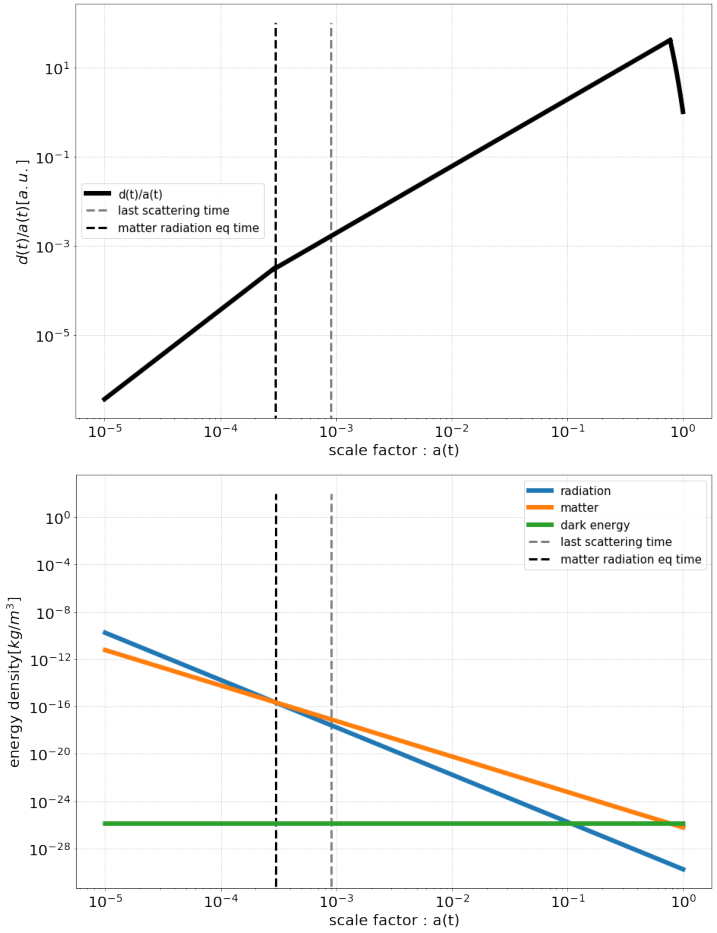
\includegraphics[width=1\columnwidth]{2_cosmology/figs/scale_dev2.pdf}
  \caption{粒子の地平線の共同距離(上図)とエネルギー密度(下図)の時間発展。
  粒子の地平線の共同距離は現在時刻の値を~1~として正規化している。
  物質とダークエネルギーのエネルギー密度は~Plank~の観測結果\cite{plank}を用い、
  放射のエネルギー密度は~CMB~の温度~(T = 2.725K)~と現存するニュートリノが全て放射として振舞うとして計算した。}
  \label{scale_dev}
\end{figure}
図~\ref{scale_dev}~から分かるように放射、物質優勢期では粒子の地平線は
宇宙の膨張に比べて早く広がるため、相関を持つ領域は広がる。
CMB~は最終散乱時刻での散乱光なので、その時の地平線距離は見込み角度にして~$2^{\circ}$である。
つまり、$2^{\circ}$以上離れた領域同士では相関を持てないことになる。
しかし、宇宙のどの方向からの~CMB~も$10^{-5}~{\rm K}$~の精度で同じ温度であることが
観測されている。
このように、相関を持つ必然性のない領域まで温度が一致している理由をビッグバン宇宙論では説明できない。
このことは、「地平線問題」と呼ばれている。


%\subsection{平坦性問題}


\section{インフレーション理論とCMBの偏光}

地平線問題をはじめとする現在のビッグバン宇宙論の種々の問題を解決する有力な理論模型がインフレーション理論である\cite{sato}。
この理論は宇宙初期のビッグバン期より前に時空が加速膨張したとする理論である。
そして、その際に原始重力波が生成されることが予言されている\cite{gwave}。
この原始重力波は~CMB~の偏光分布に~B~モードと呼ばれる空間非対称パターンを生み出すため、
B~モードを測定することでインフレーション理論の検証ができると考えられている\cite{gwave}。
この節ではインフレーション理論と原始重力波によって生じる~CMB~の偏光パターンについて述べる。

\subsection{インフレーション理論}
図~\ref{scale_dev}~のダークエネルギー優勢期と同様に、宇宙の初期にも加速膨張があれば、粒子の地平線の共同距離は
小さくなる。宇宙初期に相関を持つことができるので、地平線問題は解決される。
宇宙が加速膨張するためには、$\ddot{a}~>~0$~であればよく、
式~(\ref{friedmann_eq})~から~$3P+\rho~>~0$が要請される。
表~\ref{energy_table}~にあるように、膨張率~$H=\frac{\dot{a}}{a} = $一定が指数関数的に膨張する条件である。

インフレーションはインフラトンと呼ばれる実スカラー場によって記述される。
インフラトンのポテンシャルを~$V(\phi)$~とするとラグランジアンとハミルトニアンは

\begin{equation}
  \mathcal{L} = a(t)^3\left[\frac{\dot{\phi}^2}{2} -V(\phi)\right]
  \label{lagrange}
\end{equation}

\begin{equation}
  \mathcal{H} = \frac{\dot{\phi}^2}{2} + V(\phi)
  \label{hamilton}
\end{equation}
と表され、式(\ref{lagrange})をオイラーラグランジュ方程式に適用すると実スカラー場の運動方程式から

\begin{equation}
  \ddot{\phi} + 3H\dot{\phi} + V^\prime(\phi) = 0
  \label{phi_eq}
\end{equation}
と求まる。ここで~$\dot{\phi} = \frac{d\phi}{dt}$、$V^\prime(\phi) = \frac{dV}{d\phi}$~である。
この方程式は摩擦をうける粒子の運動を記述する~1~次元の方程式と同じであり、$H$~が摩擦係数の役割を果たしている。
ここで、$V^{\prime}(\phi)$~と~$\ddot{\phi}$~が~$3 H \dot{\phi}$~よりも十分小さければ($V^{\prime}(\phi)$、$\ddot{\phi} \ll 3H\dot{\phi}$)、
ポテンシャルはゆっくり変化する。

式(\ref{hamilton}),(\ref{phi_eq}),(\ref{energy_eq2})からインフラトンのエネルギー密度($\rho_{\phi}$)と圧力($P_{\phi}$)は

\begin{equation}
  \rho_{\phi} = \frac{\dot{\phi}^2}{2} + V(\phi)
\end{equation}

\begin{equation}
  P_{\phi} = \frac{\dot{\phi}^2}{2} - V(\phi)
\end{equation}
と求まる。ここでポテンシャル~$V(\phi)$~よりもインフラトンの変化~($\dot{\phi}$)~が十分に小さいという
~($\dot{\phi}^2 \ll V(\phi)$)~条件を課すと~$P_{\phi} = -\rho_{\phi}$
~と近似でき、
ダークエネルギー優勢期と同様に加速膨張がおこる。
したがって、$\dot{\phi}^2 \ll V(\phi)$、$\ddot{\phi} \ll 3H\dot{\phi}$~がなりたてば、
加速膨張が長時間おきるため、宇宙初期に宇宙の全体が相関を持つことができる。
これらの条件を「スローロール条件」といい、
この条件下のインフレーションをスローロール・インフレーションと呼ぶ。
これは最もシンプルなインフレーションモデルとして知られている。


\subsection{CMBの偏光パターン}
CMB~の偏光は電子とのトムソン散乱によって生じる(図~\ref{pol1})。
実際は四方からくる~CMB~が散乱されるため、温度が一様であればあらゆる向きの偏光の重ね合わせとなり、観測者は偏光した~CMB~を観測できない。
しかし、CMB~温度揺らぎがあれば偏光が観測される(図~\ref{pol2})。
温度揺らぎは物質と光子の密度揺らぎから生じる。
密度が高い領域では重力赤方偏移が強いため、CMB~の温度が最終散乱時刻における温度よりも低くなり、
密度が低い領域では~CMB~の温度は相対的に高くなる。


\begin{figure}[htbp]
  \centering
  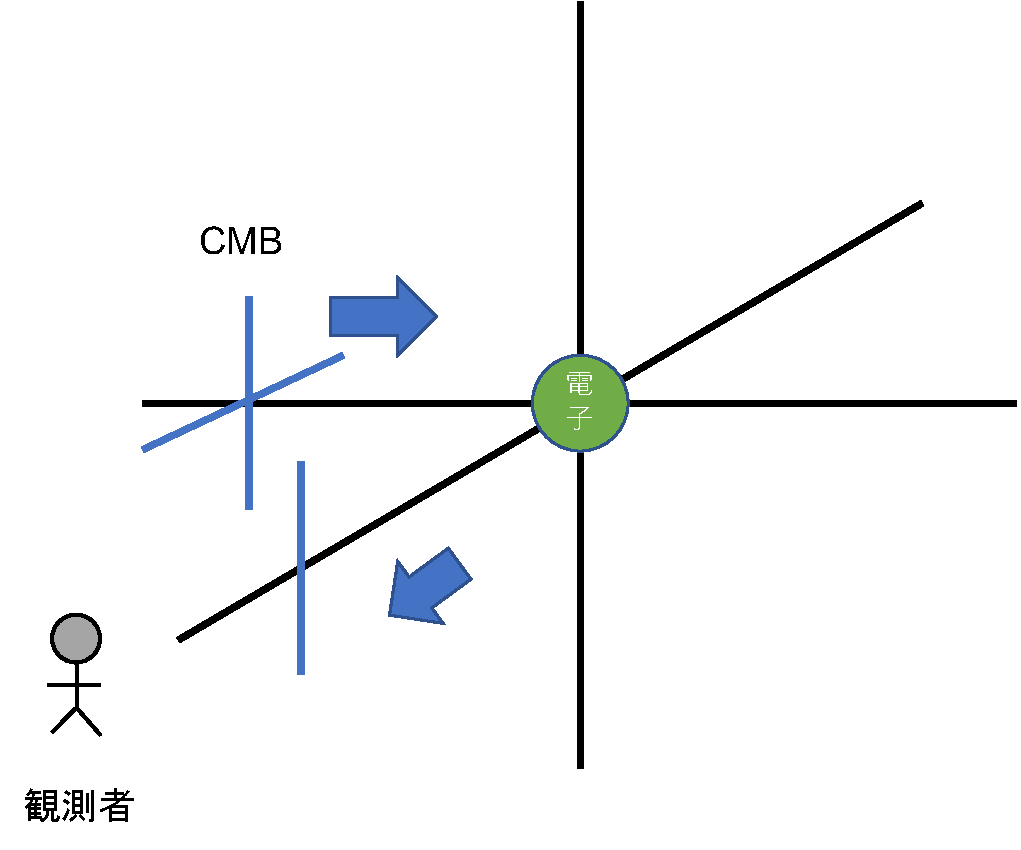
\includegraphics[width=0.8\columnwidth]{2_cosmology/figs/pol1.pdf}
  \caption{偏光が生み出される原理。
  電子の静止形で考えており、青線は~CMB~の偏光の向きを表している。
  電子と散乱する前は様々な偏光の向きを持っているが、進行方向に対して垂直方向に散乱された時
  は散乱後の進行方向の偏光成分しか残らないため、CMB~は偏光する。}
  \label{pol1}
\end{figure}

\begin{figure}[htbp]
  \centering
  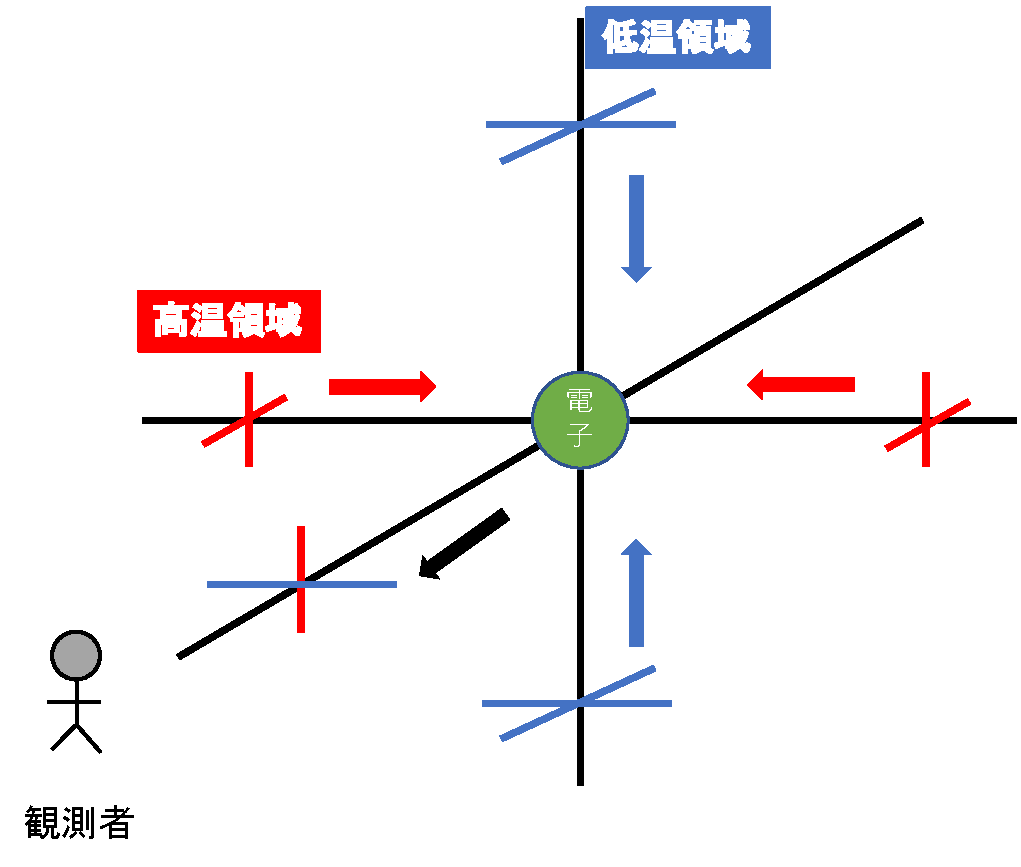
\includegraphics[width=0.8\columnwidth]{2_cosmology/figs/pol2.pdf}
  \caption{温度揺らぎから偏光が生じる原理。
  高温領域からの~CMB~の強度の方が低温領域からの強度よりも低いので、
  低温領域から散乱される~CMB~によって生じる偏光方向を持つ~CMB~が観測される。}
  \label{pol2}
\end{figure}


%観測者を中心とする曲座標空間で、偏光の方向を定義する。
実際に観測できる量はアンテナが感度を持つ方向の電場の強度($E_x, E_y$)である。
温度マップは~2~次元の和($\sqrt{E_x^2 + E_y^2}$)で作ることができる。
CMB~の偏光成分は~$x-y$~方向の直交成分とそれを~$45^{\circ}$回転させた成分の2つが考えられる。
これらの観測量は観測者の系によって変化する量なので、観測者の系によらない物理量として偏光成分を区別する必要がある。
そこで、揺らぎの進行方向に対して空間対称な偏光成分を~E~モード、
空間非対称な偏光成分を~B~モードと定義して区別する(図\ref{ebmode1})。
このように偏光成分を定義することで、どこで観測しても同じ物理量として評価できる。
密度揺らぎが作る温度揺らぎは空間対称なので、密度揺らぎは~E~モードしか生成しない。
そのため、B~モードを生成する要因は限られている。

\begin{figure}[htbp]
  \centering
  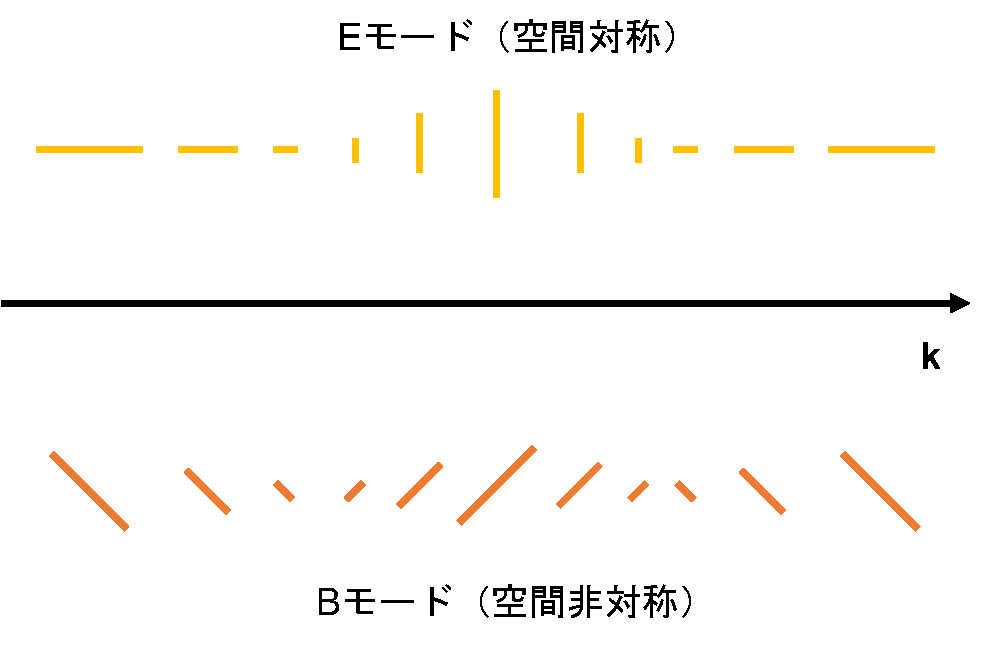
\includegraphics[width=0.8\columnwidth]{2_cosmology/figs/ebmode1.pdf}
  \caption{揺らぎの方向(k)に対するE~モードと~B~モード偏光成分。色付きの直線が偏光の方向と大きさを表す。}
  \label{ebmode1}
\end{figure}

\begin{figure}[htbp]
  \centering
  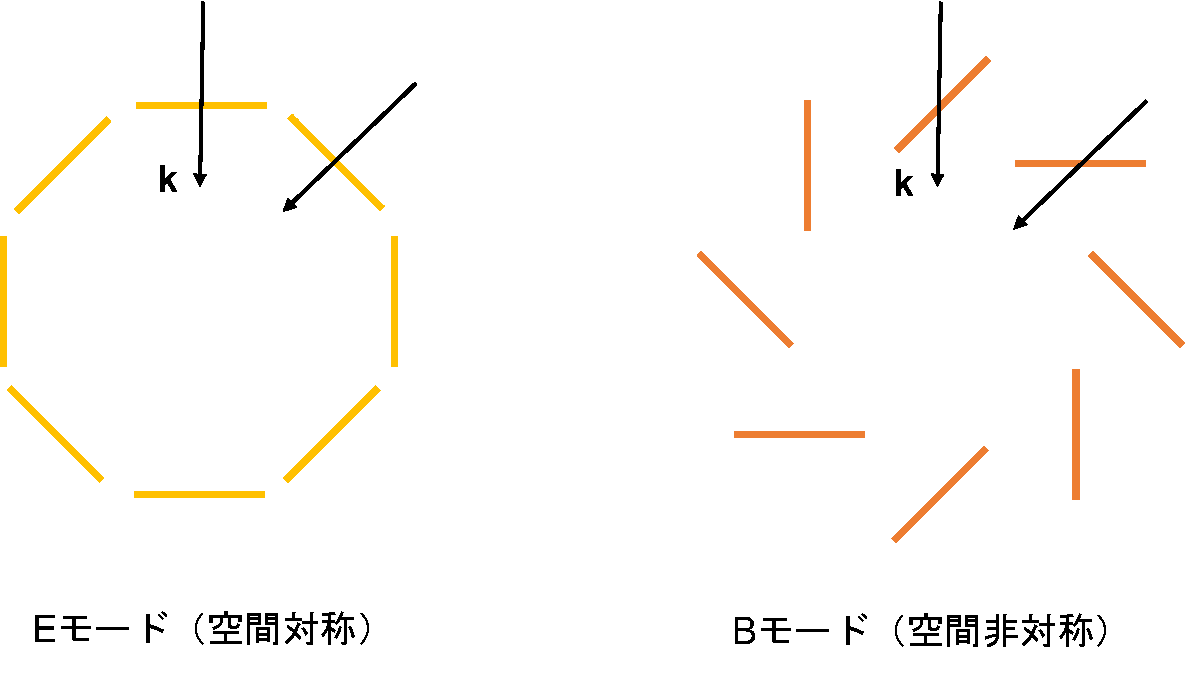
\includegraphics[width=0.8\columnwidth]{2_cosmology/figs/ebmode2.pdf}
  \caption{様々な方向の揺らぎを重ね合わせたE~モードと~B~モード偏光成分。}
  \label{ebmode2}
\end{figure}

\subsection{CMB~の偏光観測から求まる物理量と現在の観測精度}

B~モードを生み出す要因は
\begin{itemize}
  \item 原始重力波
  \item 大規模構造による重力レンズ効果
\end{itemize}
の2つが考えられる。
前者は原始重力波によるテンソル型のゆらぎが時空を変化させて作った四重極の温度異方性と電子の散乱によって生じる~B~モードである。
後者は最終散乱時刻に散乱されて生じた~E~モードが重力レンズ効果によって、その偏光軸が回転することによって生じる。
これらはパワースペクトルの~$\ell$~依存性の違いから区別できる(図~\ref{cl_shonda})。

\begin{figure}[htbp]
  \centering
  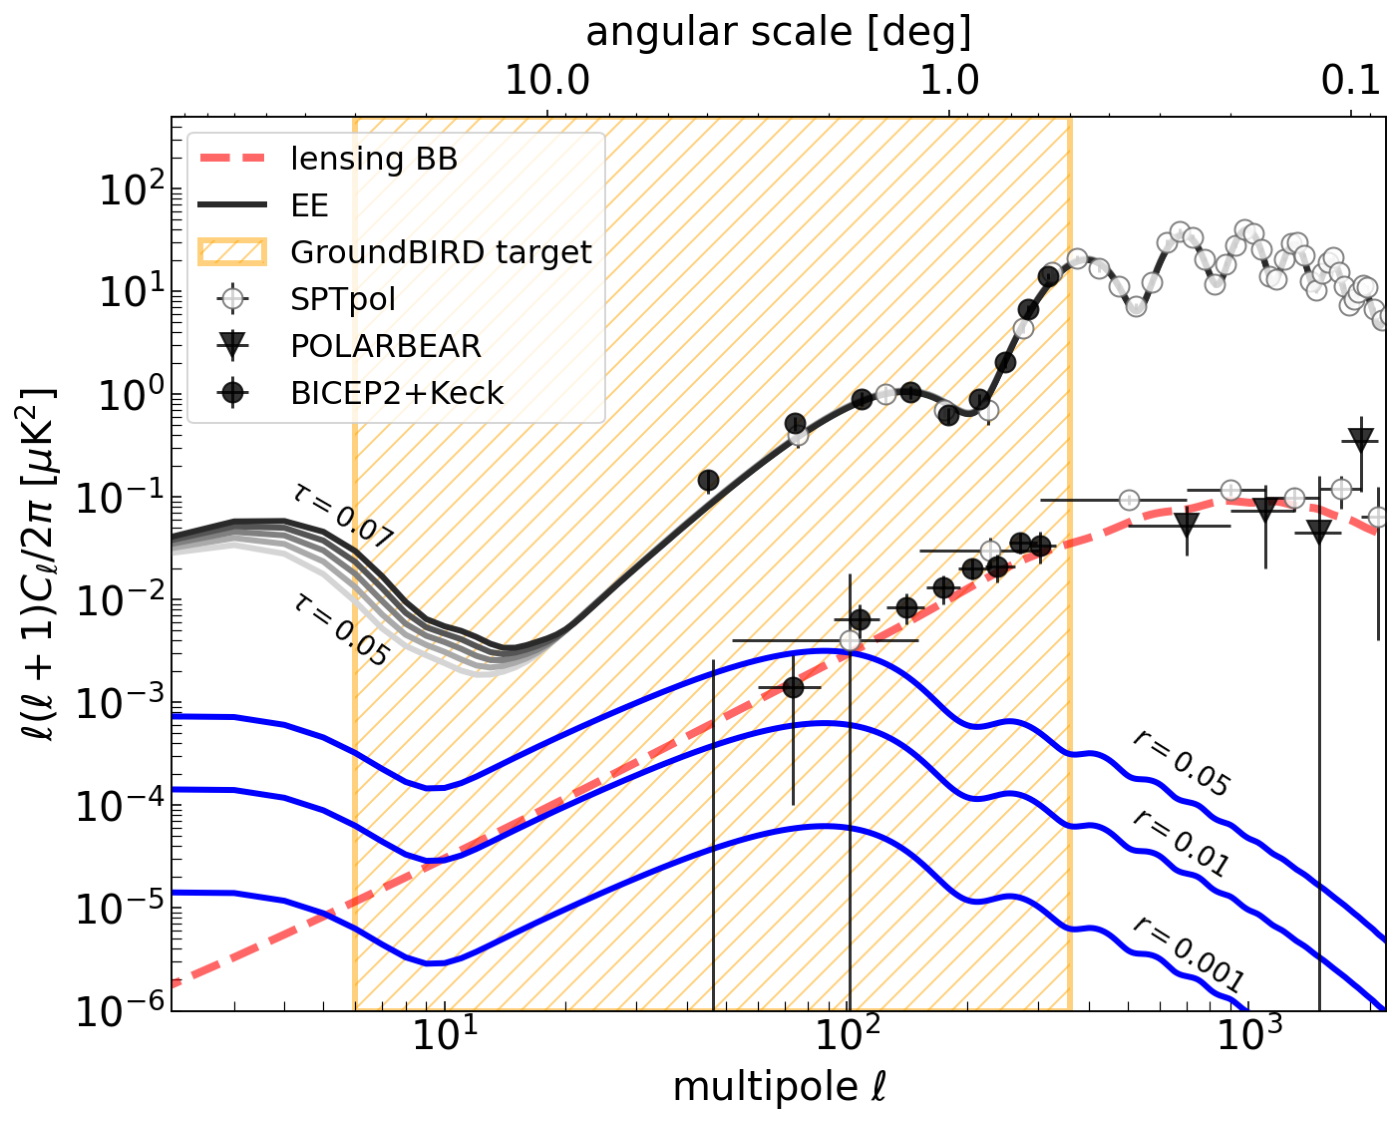
\includegraphics[width=0.8\columnwidth]{2_cosmology/figs/cl_shonda.pdf}
  \caption{過去の観測データと~E,B~モードの理論線、並びに~GroundBIRDの観測領域\cite{shonda_spie}。
  青実線は各テンソル・スカラー比での原始重力波由来の~B~モード、
  赤点線は重力レンズ効果による~B~モードを表す。
  黒実線は~E~モードを表しており、大角度スケール($\geq 10^{\circ}$)で~$\tau$~による違いが現れる。}
  \label{cl_shonda}
\end{figure}
原始重力波の発見はインフレーションの決定的な証拠となるため、CMB~研究者の悲願である。
図~\ref{cl_shonda}~から分かるように、原始重力波の探索は重力レンズ効果の~B~モードの少ない、比較的大きな角度スケールで行う必要がある。
原始重力波のテンソル型の振幅はスカラー型のゆらぎの振幅との比で表される。
この値をテンソル・スカラー比~$r$~と呼び、

\begin{equation}
  r(q) = \frac{4P_{重力波}(q)}{P_{スカラー}(q)}
  \label{tenserscalar}
\end{equation}
で定義される。ここで$P_{重力波}(q)とP_{スカラー}(q)$はそれぞれ原始重力波とスカラー型ゆらぎのパワースペクトルである。
現在はPlank~実験と~BICEP2/Keck~Array~実験による観測結果を組み合わせたものが、~$r$~に対して
\begin{equation}
  r(q = 0.002) < 0.056~(95\%~{\rm Confidence~Level})
\end{equation}
と最も厳しい制限を与えている\cite{plank}。


\begin{figure}[htbp]
  \centering
  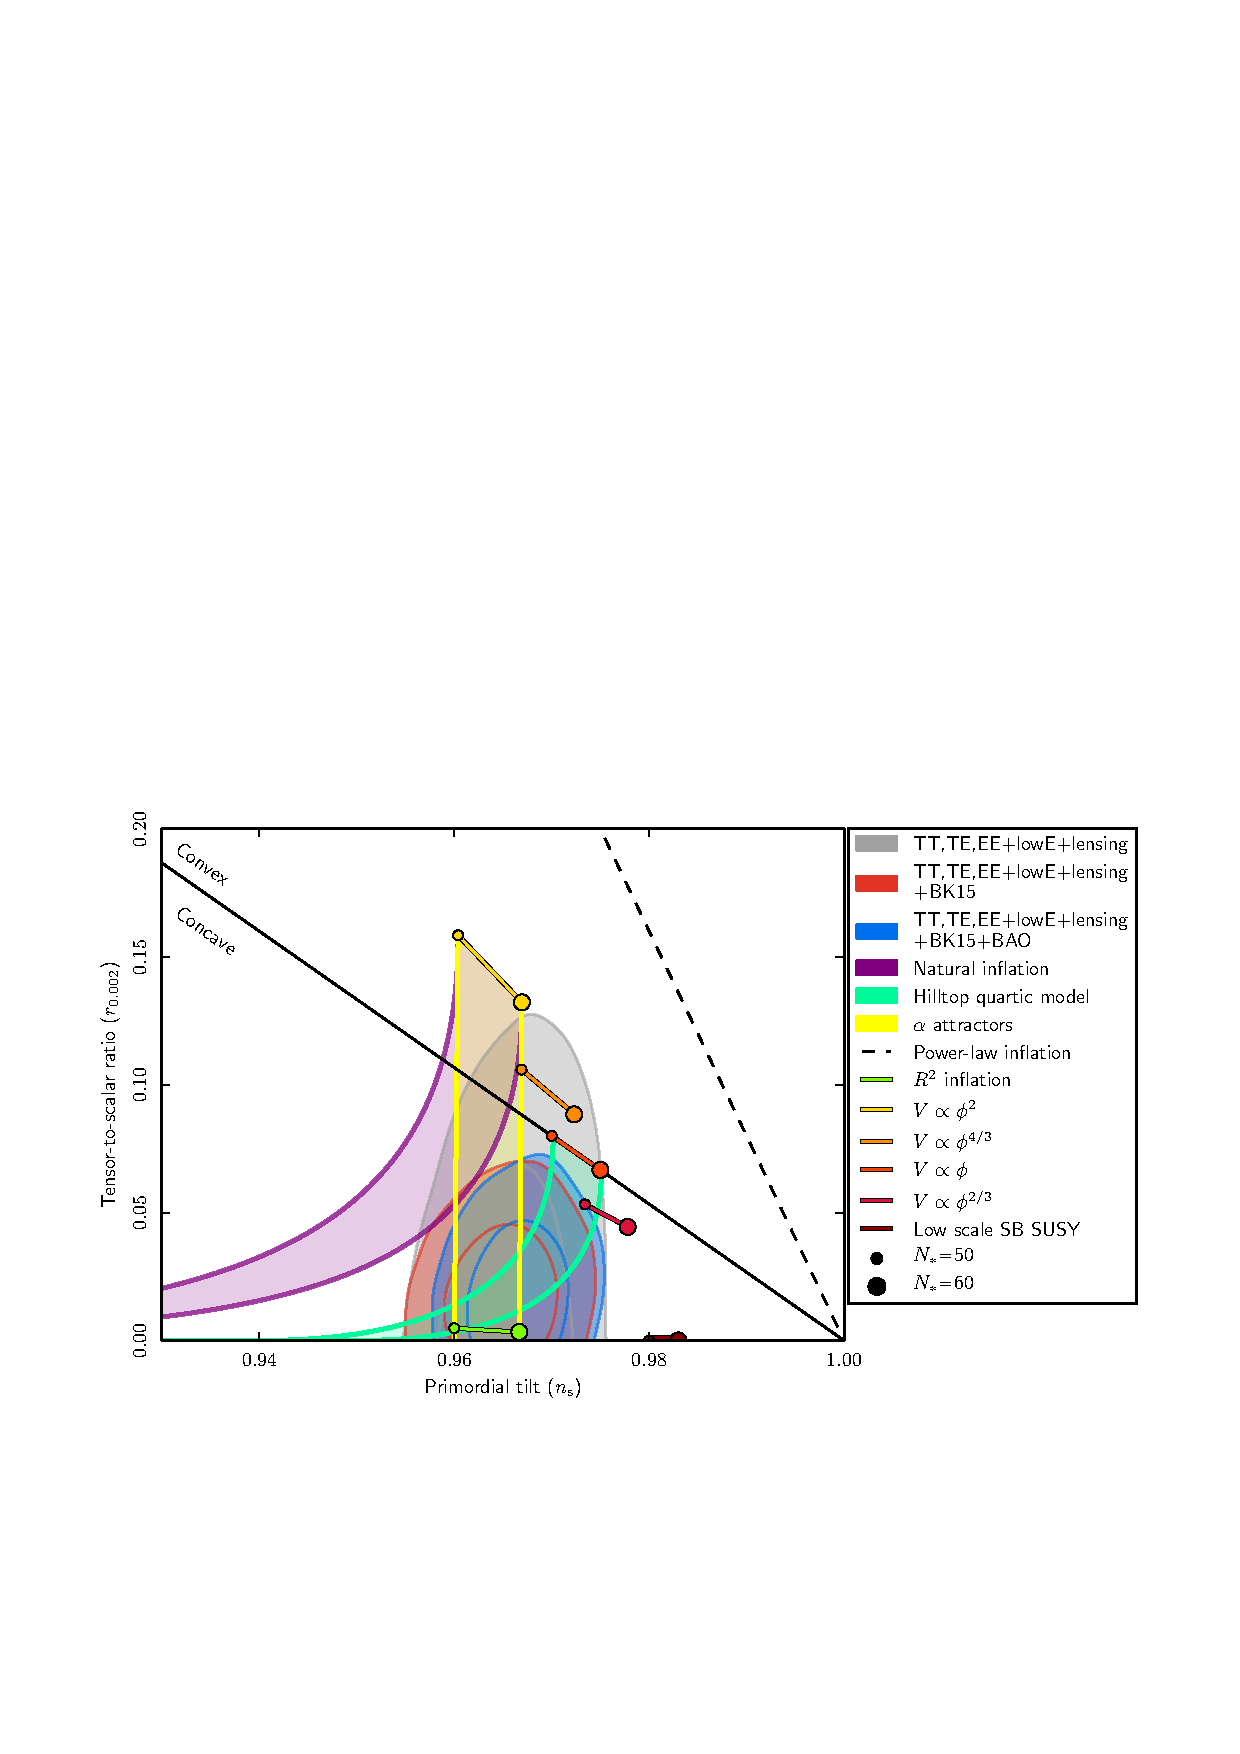
\includegraphics[width=1\columnwidth]{2_cosmology/figs/plank_r.pdf}
  \caption{Plank~実験によって与えられた~$r$,~$n_s$と平面に付けられた制限\cite{plank}。
  $n_s$~はスカラー型原始ゆらぎのべき係数を表しており、1~からずれていることはインフレーションを支持していると考えられる。
  また、いくつかの理論モデルの予測値も書かれており、それらはインフレーション期間($t_{*}<t<t_{end}$)でのスケール因子の膨張率($N_* \equiv \ln\frac{a(t_{end})}{a(t_*)}$)~
  の不定性($50<N_*<60$)を含んだものとして表されている。}
  \label{ebmode2}
\end{figure}


一方、小角度スケールの重力レンズ効果による~B~モード観測から、
ニュートリノ質量の総和($\Sigma m_{\nu}$)を求めることができる。
ただし、観測される~B~モードの強度は再電離期における光学的厚み($\tau$)と強く相関しているため、その縮退を解かねばらない。
再電離期とは、宇宙に中性水素を電離することのできるエネルギーをもつ天体が形成された以降の時期であり、
天体からの放射で中性水素から電離した電離電子が再び宇宙の中に増えていく。
これによって、小角度スケール($\ell \sim 1000$)で観測される重力レンズ効果の偏光パターンは弱められる。
他方、CMB~と電子の新たな散乱によって、新たな偏光パターンが大角度スケール($\ell < 10$)に生成される。
前者の理由で~$\tau$~と~$\Sigma m_{\nu}$~は縮退し、後者の理由から~$\tau$~を測定する最良の手段が、大角度スケールの~E~モード測定となる(図~\ref{cl_shonda})。

したがって、大角度の~E~モードの精密観測を行うことで、ニュートリノ質量和($\Sigma m_{\nu}$)の測定精度を向上できる。
例えば、$\tau$~の測定精度が~$\sigma (\tau) \approx 0.01$~となれば、$\Sigma m_{\nu}$~の測定精度は~$\sigma (m_{\nu}) \approx 120~{\rm meV}$~となる\cite{plank}。

\section{GroundBIRD~実験}
GroundBIRD~実験は大角度スケールの~CMB~偏光パターン測定に特化した実験である。
図~\ref{gb}~にGroundBIRDの望遠鏡の概要を示す。

\if0
\begin{figure}[h]
  \begin{subfigure}[left]{0.4\columnwidth}
    \centering
    \includegraphics[width = 0.4\columnwidth]{2_cosmology/figs/groundBIRD2.png}
    \caption{GroundBIRD~望遠鏡の外観}
  \end{subfigure}
  \centering
  \begin{subfigure}[right]{0.6\columnwidth}
    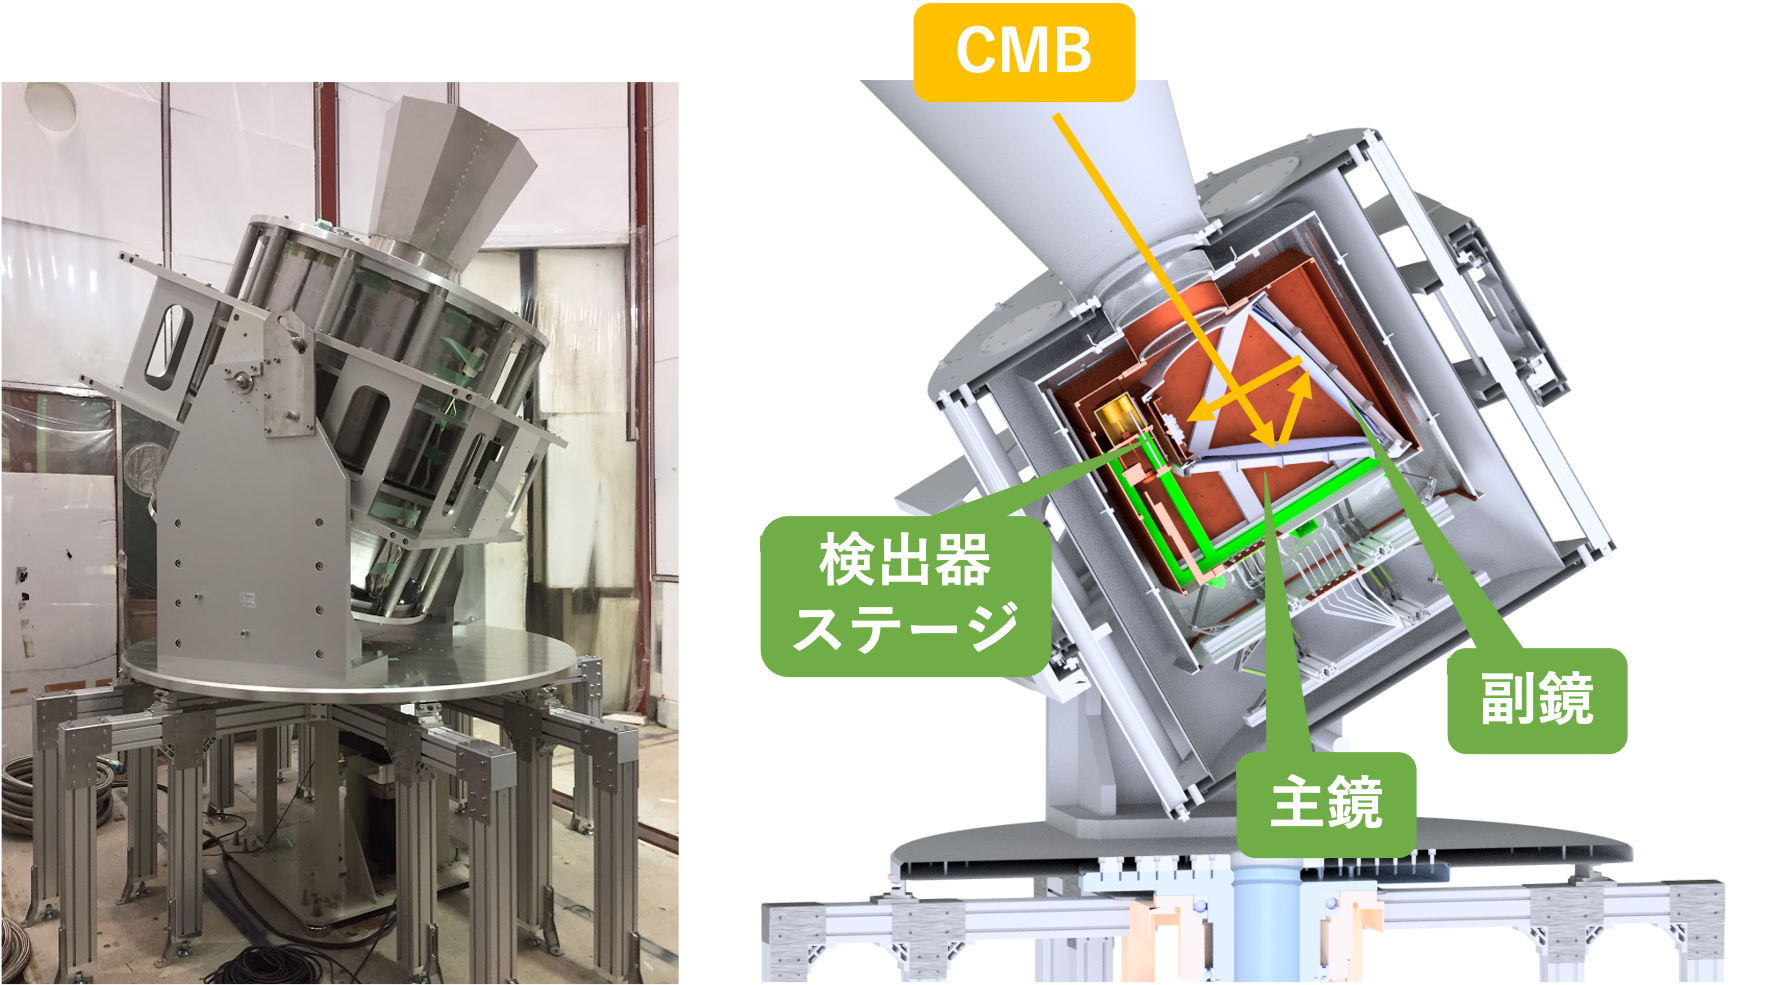
\includegraphics[width = 0.6\columnwidth]{2_cosmology/figs/gb1.png}
    \caption{GroundBIRD~望遠鏡の内部構造バッフルから入ってきた~CMB~が主鏡、副鏡の順に反射され、検出器ステージに入る}
  \end{subfigure}
  \caption{GroundBIRD~望遠鏡}
\end{figure}

\begin{figure}[h]
  \begin{tabular}{cc}
    %---- 最初の図 ---------------------------
    \begin{minipage}[t]{0.3\hsize}
      \centering
      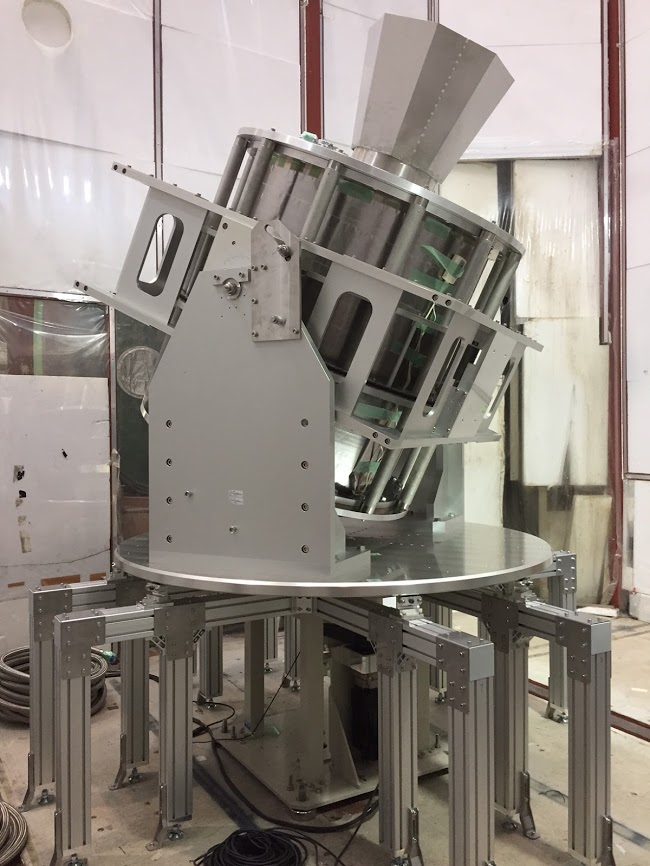
\includegraphics[keepaspectratio, scale=0.2]{2_cosmology/figs/GroundBIRD2.png}
    \end{minipage} 
    %---- 2番目の図 --------------------------
    \begin{minipage}[t]{0.65\hsize}
      \centering
      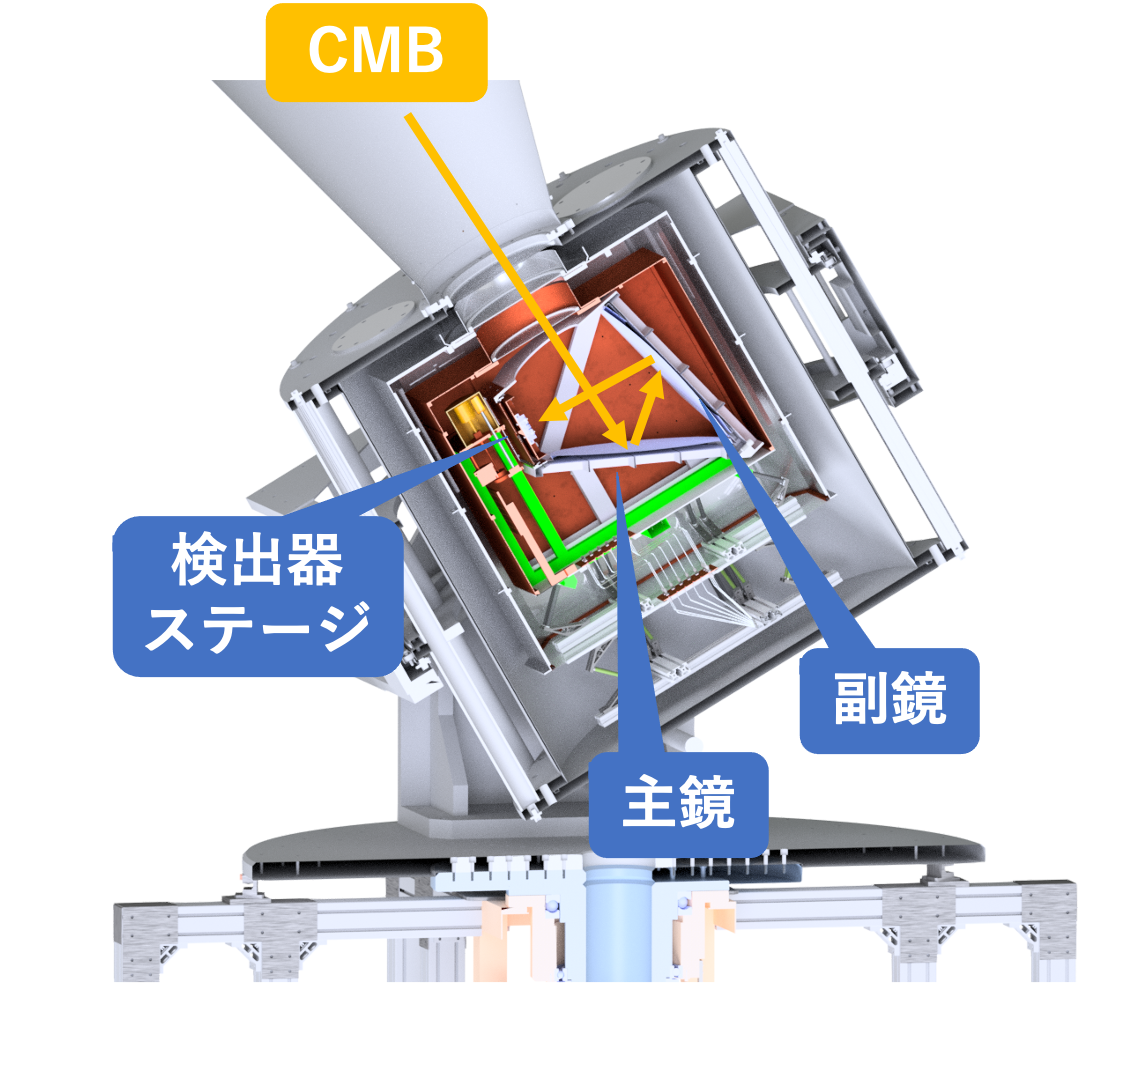
\includegraphics[keepaspectratio, scale=0.35]{2_cosmology/figs/gb_int.png}
    \end{minipage}
    %---- 図はここまで ----------------------
  %\caption{GroundBIRDの概要}
  \end{tabular}
  \caption{GroundBIRD~望遠鏡の外観の写真と概念図。バッフルから入ってきた~CMB~が主鏡、副鏡の順に反射され検出器ステージに入る。}
  \label{gb}
\end{figure}
\fi

\begin{figure}[htbp]
  \centering
  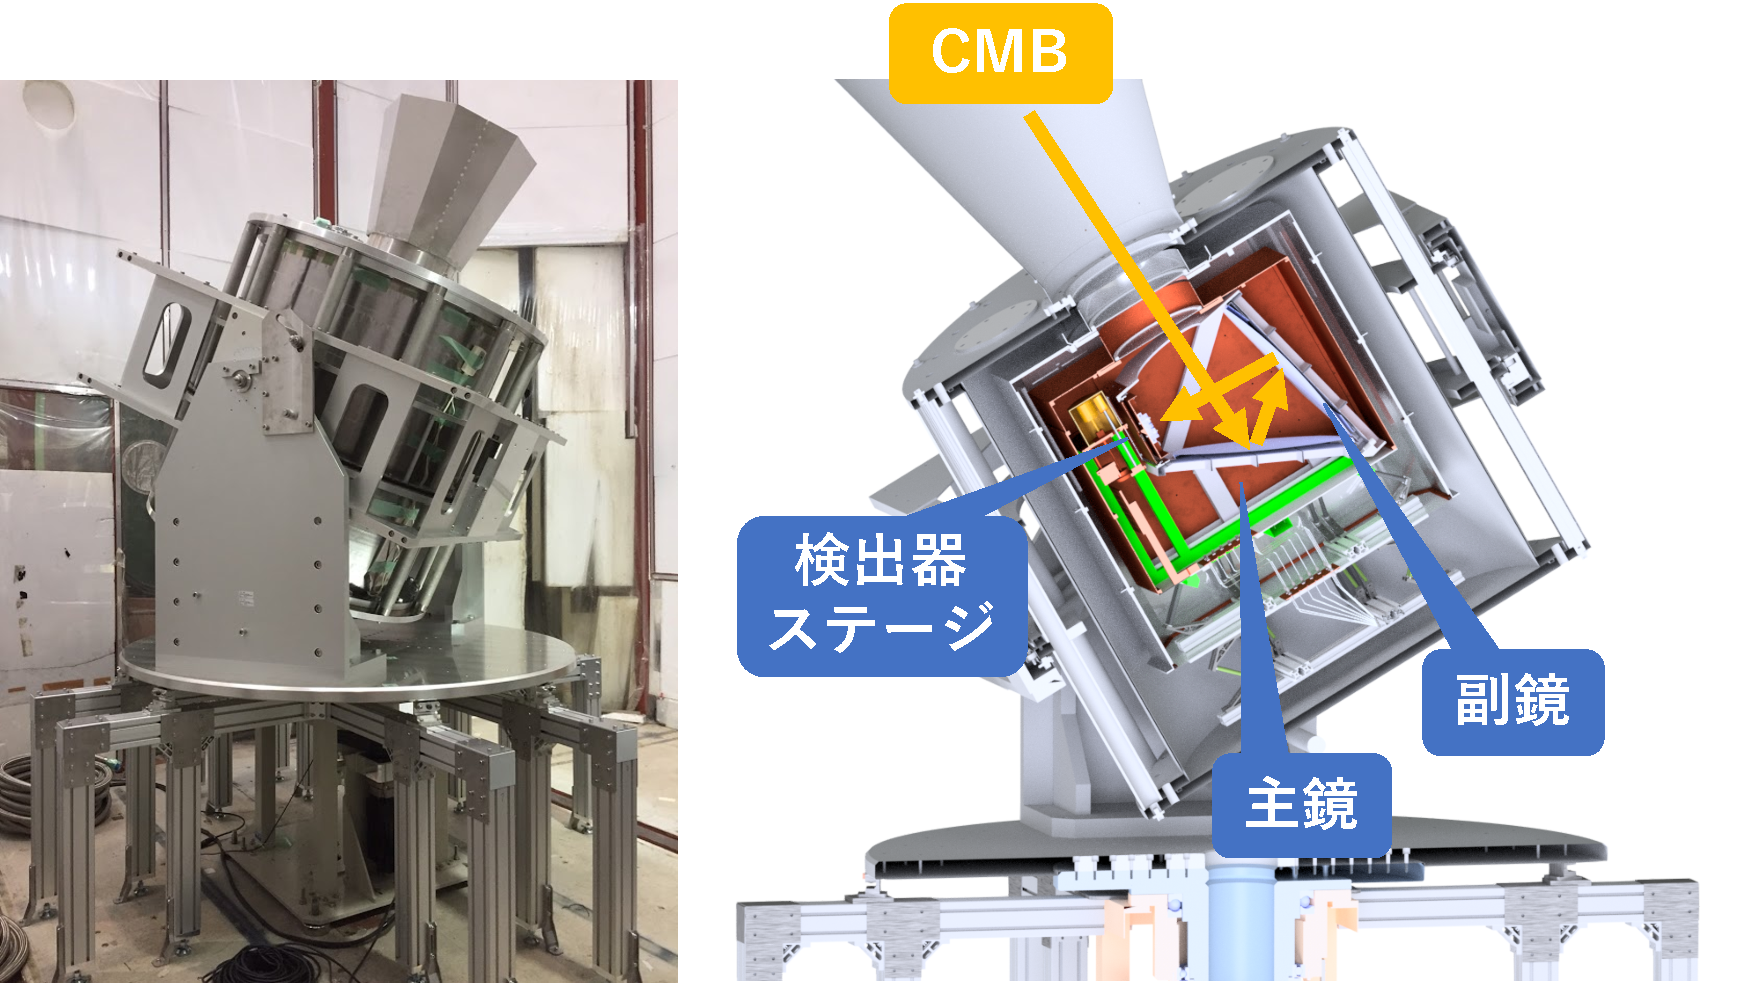
\includegraphics[width=1\columnwidth]{2_cosmology/figs/gb.pdf}
  \caption{GroundBIRD~望遠鏡の外観の写真と概念図。バッフルから入ってきた~CMB~が主鏡、副鏡の順に反射され検出器ステージに入る。}
  \label{gb}
\end{figure}

地上からの観測において最も邪魔になるのが大気の放射であるが、
大気の放射は無偏光であるため、地上から~CMB~の偏光を観測することが可能である。
しかし、観測装置の不完全性によって無偏光を偏光と見誤る影響が無視できない(典型的には~1\%~未満の影響)。
つまり、大気の揺らぎ(継時変化)の影響を抑制するための変調が必要である。
GroundBIRD~では、望遠鏡を3秒で一回転させる独自の高速スキャンストラテジーで大気揺らぎの影響を抑制しながら観測を行う。
望遠鏡を天頂方向から~$30^\circ$~傾けて回転させることで、地球の自転と相まって、1~日で全天の~$45\%$~の領域の観測を実現する。
そして、角度分解能は~$0.6^{\circ}$(FWHM)であるので、
GroundBIRDは~6~$\textless$~$\l$~$\textless$~360~の領域を測定する(図~\ref{cl_shonda})。
先の節で述べたように、原始重力波と再電離期の光学的厚み~$\tau$~の測定に最適化した実験戦略である。
GroundBIRD~の高速スキャンのもとで角度分解能を失わないために、検出器は応答時間が~5~ミリ秒以下であることが必要である。
そのため、GroundBIRD~では~``MKID"~という超伝導検出器を導入する。
MKID~の典型的な応答時間は~1~ミリ秒以下なのでこの要求を満たす。
%GroundBIRD~の検出器ステージには~145GHz~,~225GHz~帯域の検出器が

MKID~に由来するノイズの特性には、以下のことが要求される。
\begin{itemize}
  \item MKID~固有のノイズが観測環境下において入射する大気の熱放射ノイズよりも低いこと
  \item MKID~固有の~$1/f$~ノイズの~knee~frequency~がスキャン周期(0.3~Hz)よりも低いこと
\end{itemize}

$1/f$~ノイズとは観測時間に比例して大きくなるようなノイズの総称である。
測定時の周波数が大きくなるほど小さくなるノイズなので、$1/f$~ノイズと呼ばれる(図~\ref{noise_example})。
検出器の出力信号のベースラインがゆっくりと時間変動して揺らぐことが、そのようなノイズ成分を作り出す。
MKID~における~$1/f$~ノイズの主要因が後述する~TLS~ノイズである。
なお、自然界にはこのようなノイズ成分が多く存在する。例えば、大気放射の時間変動も~$1/f$~ノイズである。
また、knee~frequency~とは時間依存しないノイズ成分(ホワイトノイズ)と~$1/f$~ノイズが同程度の寄与となる周波数のことであり、
本論文では``\fknee''と定義する。

製作した~MKID~が上記の性能を満たす事を観測に先立って把握しておくことは、実験を行う上で非常に重要である。
本論文では、第~2~章で~MKID~の原理、読み出し手法、ノイズ成分について述べた後、
望遠鏡への搭載に先立って~MKID~の特性を理解する評価系の構築を行う(第~3~章)。
そして、開発した評価系を用いて従来の~MKID~の~TLS~ノイズについての定量的な評価を行う(第~4~章)。
その後、従来に比べて~TLS~ノイズを低減できる~MKID~デザインを考案し、その定量的な評価を行う(第~5~章)。
最後に本研究のまとめと今後の展望について述べる。


\begin{figure}[htbp]
  \centering
  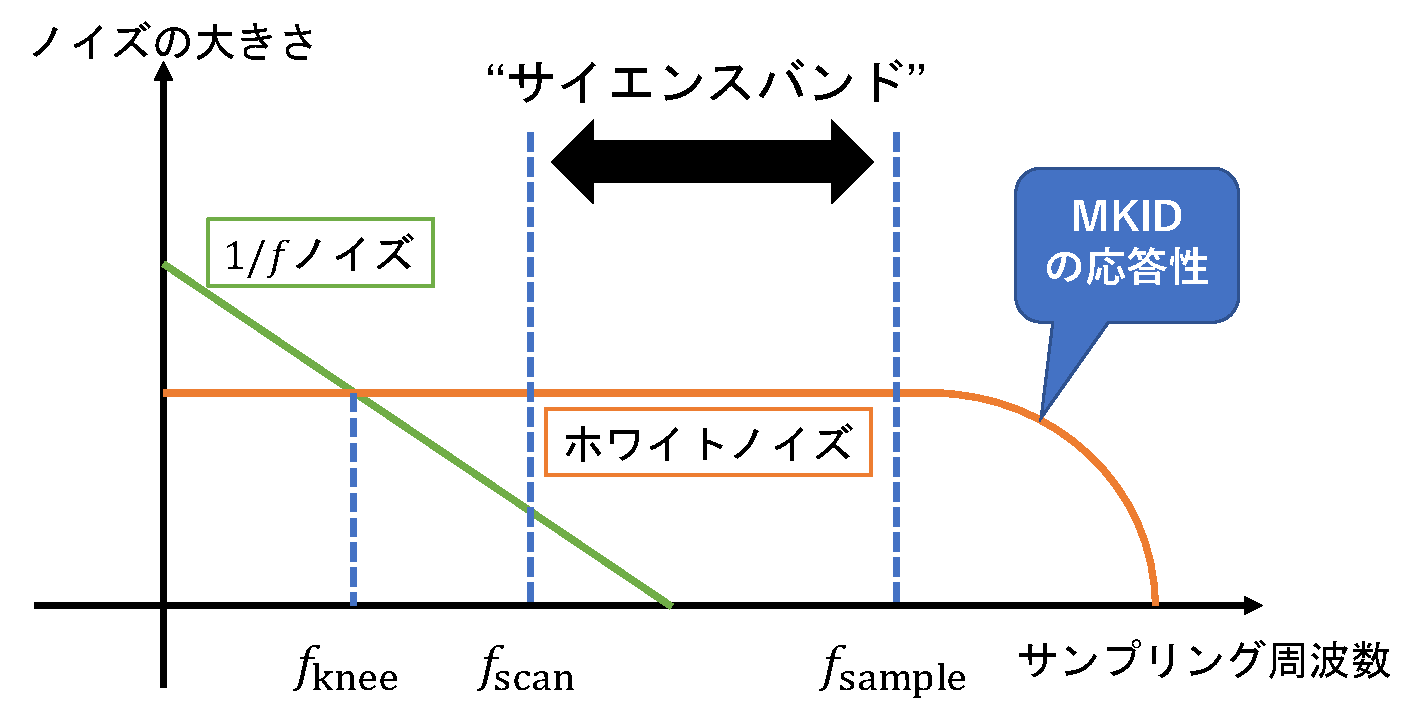
\includegraphics[width=1\columnwidth]{2_cosmology/figs/noise_example.pdf}
  \caption{スキャン周期($f_{\rm scan}$)、サンプリング周期($f_{\rm sample}$)と~MKID~のノイズ特性の理想的な関係。
  $f_{\rm knee} < f_{\rm scan}$~であること、つまり「サイエンスバンド」($f_{\rm scan}~ から~ f_{\rm sample}$~までの周波数)に~$1/f$~ノイズの影響がないことが理想的な観測環境であり、
  GroundBIRD~では$f_{\rm scan} \sim 0.3~{\rm Hz}$~である。
  また、角度分解能を損なわない頻度($360^{\circ}/f_{\rm sample} \ll \Delta \theta(0.6^{\circ})$)でデータを取得し続けることも必要であり、
  GroundBIRD~では$f_{\rm sample} = 1~{\rm kHz}$~である。}
  \label{noise_example}
\end{figure}
\include{3_MKID/MKID}
\include{4_MKIDkyoto/MKIDkyoto}
\include{5_TLS/TLS}
\include{5_TLS/TLS_wide}
\include{6_Summary/Summary}
%

% 謝辞
\chapter{謝辞}

本修士論文の執筆にあたり、多くの方々にご支援いただきました。
ご支援いただいた全ての方々にこの場を借りてお礼申し上げます。
この~2~年間は非常に有意義なもので、大いに成長できたと思います。


指導教員である田島治准教授には、CMB~という魅力的なテーマと、研究を行う上でこれ以上ない環境を作っていただきました。
研究も基本的には自由にやらせていただいて、とても楽しく、やりがいがありました。
また、数多くの的確な助言などで研究を正しい道に導いていただきました。
修士論文の作成にも多大なる時間と労力を割いていただきました。
文章を書くのが下手な私も無事に修士論文を書き終えることができたのは、田島さんの尽力のおかげです。
本当にありがとうございます。

GroundBIRD~実験のメンバーの皆様にも感謝申し上げます。
鈴木惇也助教にはデバイス扱い方から本修士論文の内容まで、私の研究のほぼ全てにおいてサポートしていただきました。
研究が詰まった時は、よく相談にも乗っていただき、ミーティングでも毎回的確な助言をいただきました。
本多俊介氏には読み出し回路や~GroundBIRD~実験について数多く教えをいただきました。
夜遅くまで私の研究を手伝っていただくこともありました。
また、よくコーヒーにも誘っていただき、良いリフレッシュをすることができました。
東北大学の沓間弘樹氏には~MKID~について非常に多くのことを教えていただきました。
修士論文の内容についても相談に乗っていただき、多くの助言をいただきました。
%良いものになったのも沓間さんの力が大きいです。
どんな質問でも嫌がらず、丁寧に説明してくれました。
私の~MKID~の基礎は沓間さんによって作られたと言っても過言ではありません。
池満拓司氏には~MKID~の測定手法の基本を教わりました。
%池満さんの着実に研究を進める様子は非常に魅力的でした。
また、テネリフェでは海に連れて行っていただくなど、テネリフェでの私生活でもお世話になりました。
小栗秀悟助教、長崎岳人氏にはテネリフェで~GroundBIRD~望遠鏡について様々なことを教わりました。
理研の美馬覚氏には冷凍機と~MKID~について助言をいただきました。

京都~CMB~グループの皆様にもお世話になりました。
安達俊介氏には冷凍機の立ち上げからその運用に関して多くの助言を多くいただきました。
大塚稔也君には研究を行う上で毎日、非常に刺激を受けました。
先々のことを見据え、着実に研究を進める大塚君が同期にいたことは私の研究姿勢にも良い影響を及ぼしてくれました。
阿部倫史氏と小高駿平君、中田嘉信君にはミーティングやゼミでお世話になりました。

デルフト工科大学の遠藤光氏、SRON~の唐津謙一氏、埼玉大学の成瀬雅人氏には
MKID~の評価系を構築する上で多くの助言をいただきました。心から感謝申し上げます。

ここには書ききれませんが、研究生活の様々な場面でお世話になった先生方、先輩、後輩、秘書の皆様にも感謝申し上げます。
%のびのびと研究のできる良い研究室に恵まれたと実感しております。
また、同期の小林蓮君、菅島文悟君、谷真央君、辻川吉明君は一緒に博士課程に進学することもあり、多くの刺激をうけました。

最後に、いつも応援し、支えてくれた家族と真衣に感謝します。ありがとう。
%

% 参考文献
\begin{thebibliography}{99}
\addcontentsline{toc}{chapter}{\protect\numberline{}{参考文献}\hfil}
\markboth{\bibname}{参考文献}

% 2_introduction
\bibitem{cobe}
\href{D. J. Fixsen and E. S. Cheng and J. M. Gales and J. C. Mather and R. A. ShaFer and E. L. Wright. The cosmic microwave background spectrum from the full cobe firas data set. The Astrophysical Journal, 473(2):576, 1996.}{
D. J. Fixsen and E. S. Cheng and J. M. Gales and J. C. Mather and R. A. ShaFer and E. L. Wright. The cosmic microwave background spectrum from the full cobe firas data set. The Astrophysical Journal, 473(2):576, 1996.
}

\bibitem{cmb_discovery}
\href{https://ui.adsabs.harvard.edu/abs/1965ApJ...142..419P/abstract}{
A. A. Penzias, R. W. Wilson. A Measurement of Excess Antenna Temperature at 4080 Mc/s. {\it Astrophysical Journal}, vol.142, p.419–421, 1965.
}

\bibitem{cmb_discovery_theory}
\href{https://ui.adsabs.harvard.edu/abs/1965ApJ...142..414D/abstrac}{
R. H. Dicke, P. J. E. Peebles, P. G. Roll, D. T. Wilkinson. Cosmic Black-Body Radiation. {\it Astrophysical Journal}, vol.142, p.414–419, 1965.
}


\if0
\bibitem{wmap}
\href{https://map.gsfc.nasa.gov/}{
https://map.gsfc.nasa.gov/
}
\fi

\bibitem{shonda_spie}
\href{https://www.spiedigitallibrary.org/conference-proceedings-of-spie/11445/114457Q/On-site-performance-of-GroundBIRD-a-CMB-polarization-telescope-for/10.1117/12.2560918.short}
{S.Honda, et al., On-site performance of GroundBIRD, a CMB polarization telescope for large angular scale observations. Proceedings Volume 11445, Ground-based and Airborne Telescopes VIII; 114457Q (2020)}


\bibitem{plank}
\href{https://www.aanda.org/articles/aa/full\_html/2020/09/aa33880-18/aa33880-18.html}
{Planck Collaboration, Plank 2018 results. 1.Overview and the cosmological legacy of Planck. Astronomy \& Astrophysics, 2018.}

\bibitem{sato}
\href{https://ui.adsabs.harvard.edu/abs/1981MNRAS.195..467S/abstract}
{K. Sato. First-order phase transition of a vacuum and the expansion of the universe. Monthly Notices of the Royal Astronomical Society, Vol 195:pp.467–479, 1981.}


\bibitem{gwave}
\href{https://arxiv.org/abs/1605.01615}
{Maria Chiara Guzzetti, et al., Gravitational waves from inflation.}

\bibitem{n_mass}
\href{https://journals.aps.org/prd/abstract/10.1103/PhysRevD.92.123535}{
  R. Allison, P. Caucal, E. Calabrese, J. Dunkley, and T. Louis, Towards a cosmological neutrino mass detection. Phys. Rev. D 92, 123535, 2015.
}

% 3_MKID
\bibitem{high_eff}
\href{https://aip.scitation.org/doi/10.1063/1.4829657}{
  R. M. J. Janssen, et al., High optical efficiency and photon noise limited sensitivity of microwave kinetic inductance detectors using phase readout. Appl. Phys. Lett. 103, 203503, 2013.
}

\bibitem{microwave_eng}
D. M. Pozar. Microwave Engineering. John Wiley \& Sons, Inc., Hoboken, New Jersey, 2012.

\bibitem{BCS}
\href{https://journals.aps.org/pr/abstract/10.1103/PhysRev.108.1175}
{J. Bardeen, L. N. Cooper, and J. R. Schrieffer. Theory of superconductivity. Physical
Review, 108:1175, 1957.
}

\bibitem{fremi_dense}
\href{G. Vardulakis. Superconducting kinetic inductance dectectors: theory, simulations and
experiments. University of Cambridge, Cambridge, UK, 2007.}
{G. Vardulakis. Superconducting kinetic inductance dectectors: theory, simulations and
experiments. University of Cambridge, Cambridge, UK, 2007.
}

\bibitem{n0}
\href{https://journals.aps.org/prb/abstract/10.1103/PhysRevB.14.4854}
{S. B. Kaplan, C. C. Chi, D. N. Langenberg, J. J. Chang, S. Jafarey, et al. Quasiparticle
and phonon lifetimes in superconductors. Physical Review, B14:4854, 1976.
}

\bibitem{res_omega}
Neil W. Ashcroft, N. David Mermin. Solid State Physics

\bibitem{London}
\href{F. London and H. London. The electromagnetic equations of the supraconductor.
Proceedings of the Royal Society of London Series A, 149:71, 1935.
}{F. London and H. London. The electromagnetic equations of the supraconductor.
Proceedings of the Royal Society of London Series A, 149:71, 1935.
}

\bibitem{MS_theo}
\href{D. Mattis and J. Bardeen. Theory of the anomalous skin effect in normal and super-
conducting metals. Physical Review Letters, 111:412, 1958.}
{D. Mattis and J. Bardeen. Theory of the anomalous skin effect in normal and super-
conducting metals. Physical Review Letters, 111:412, 1958.}

\bibitem{gao}
\href{https://resolver.caltech.edu/CaltechETD:etd-06092008-235549}{
J. Gao. The Physics of Superconducting Microwave Resonators. PhD thesis, California Institute of Technology Pasadena, California, 2008.
}

\bibitem{pieter}
\href{https://doi.org/10.4233/uuid:eae4c9fc-f90d-4c12-a878-8428ee4adb4c}{
P. J. de Visser. et al., Quasiparticle dynamics in aluminium superconducting microwave resonators. PhD thesis, Delft University of Technology, Delft, The Netherlands, 2014. 
}


% 4_MKIDkyoto
\bibitem{vac_pump}
\href{http://www.hakuto-vacuum.jp/pfeiffer\_vacuum/pdf/PumpingStation/HiCubeClassic.pdf}{
http://www.hakuto-vacuum.jp/pfeiffer\_vacuum/pdf/PumpingStation/HiCubeClassic.pdf}

\bibitem{ptc}
\href{https://www.cryomech.com/products/pt407/}{
https://www.cryomech.com/products/pt407/}

\bibitem{LNA}
\href{https://www.lownoisefactory.com/products/cryogenic/lnc-4-8-ghz/}{
https://www.lownoisefactory.com/products/cryogenic/lnc-4-8-ghz/}

\bibitem{vac}
\href{https://www.pfeiffer-vacuum.com/productPdfs/PTT03140010.en.pdf}{
https://www.pfeiffer-vacuum.com/productPdfs/PTT03140010.en.pdf  
}

\bibitem{thermo}
\href{https://www.toyo.co.jp/material/products/detail/rx.html}{
https://www.toyo.co.jp/material/products/detail/rx.html
}

\bibitem{lackshore372}
\href{https://www.toyo.co.jp/material/products/detail/372.html}{
https://www.toyo.co.jp/material/products/detail/372.html
}

\bibitem{deshima_exp}
\href{http://deshima.ewi.tudelft.nl/}{
  http://deshima.ewi.tudelft.nl/
}

\bibitem{deshima}
\href{https://www.spiedigitallibrary.org/journals/Journal-of-Astronomical-Telescopes-Instruments-and-Systems/volume-5/issue-03/035004/Wideband-on-chip-terahertz-spectrometer-based-on-a-superconducting-filterbank/10.1117/1.JATIS.5.3.035004.full}{
A Endo, et al.. “Wideband on-chip terahertz spectrometer based on a superconducting filterbank“ J. of Astronomical Telescopes, Instruments, and Systems, 5(3), 035004, 2019.
}

\bibitem{deshima_image}
\href{http://aste.nao.ac.jp/pressrelease/2019deshima/index.html}{http://aste.nao.ac.jp/pressrelease/2019deshima/index.html}

\bibitem{ikemitsu}
池満拓司. CMB望遠鏡のデータ読み出しシステムの時刻同期と較正に関する開発研究. 京都大学理学研究科 修士論文 2020.

\bibitem{ishitsuka}
石塚光. 超伝導検出器 MKID の周波数多重読み出し用 フロントエンド回路の開発. 総合研究大学院大学 高エネルギー加速器科学研究科 修士論文 2020.

\bibitem{welch}
\href{https://docs.scipy.org/doc/scipy/reference/generated/scipy.signal.welch.html}{
https://docs.scipy.org/doc/scipy/reference/generated/scipy.signal.welch.html
}

\bibitem{kutsuma}
沓間弘樹. CMB偏光観測にむけた超伝導検出器”MKID”のノイズ低減法の研究開発. 東北大学理学研究科 修士論文 2018.

\bibitem{kutsuma1}
\href{https://aip.scitation.org/doi/10.1063/1.5110692}{
H. Kutsuma, et al., A measurement method for responsivity of microwave kinetic inductance detector by changing power of readout microwaves. Appl. Phys. Lett. 115, 032603, 2019.
}

\bibitem{kutsuma2}
\href{https://aip.scitation.org/doi/10.1063/5.0013946}{
H. Kutsuma, Y.Sueno, et al., A method to measure superconducting transition temperature of microwave kinetic inductance detector by changing power of readout microwaves. AIP Advances 10, 095320, 2020.
}

% 5_TLS
\bibitem{TLS_review}
\href{https://arxiv.org/abs/2006.04718}{
  C. R. H. McRae, et al., Materials loss measurements using superconducting microwave resonators. Review of Scientific Instruments 91, 091101, 2020.
}

\bibitem{kumar}
\href{https://aip.scitation.org/doi/pdf/10.1063/1.2894584?casa_token=wSixfQUGxAUAAAAA:CPs8YHoWwOGIVSeqJLakFz0-GQ9TLncU8veuICWpfjPBgZYTjr-WcUaiIv0cPRtaopytECg_taMS}{
  Shwetank Kumar, et al., Temperature dependence of the frequency and noise of superconducting coplanar waveguide resonators. Appl. Phys. Lett. 92, 123503, 2008.
}

\bibitem{rami_fexp}
\href{https://aip.scitation.org/doi/full/10.1063/1.3467052}
{R. Barends, Reduced frequency noise in superconducting resonators. Appl. Phys. Lett. 97, 033507, 2010.}

\bibitem{hybrid}
\href{https://arxiv.org/pdf/0909.2060.pdf}
{Omid Noroozian, et al., Two-level system noise reduction for Microwave Kinetic Inductance Detectors, }

\bibitem{kutsuma_D}
Hiroki Kutsuma ph.D thesis.

\bibitem{rami_cpw}
\href{https://aip.scitation.org/doi/10.1063/1.3458705}
{R. Barends, Minimal resonator loss for circuit quantum electrodynamics. Appl. Phys. Lett. 97, 023508, 2010.}

  
\end{thebibliography}

%補遺
\appendix
\chapter{Zynqへのlinux搭載}

時間あったら書きたい


%\newpage
%\chapter{MKID~forecaster}

%観測サイトにおけるシミュレーションに用いた~MKID~forecaster~の概要について述べる。


\end{document}
